\documentclass[sigconf,letterpaper,9pt]{acmart}

\newenvironment{myquote}%
  {\list{}{\leftmargin=0.3in\rightmargin=0.3in}\item[]}%
  {\endlist}

\newenvironment{glist}[3]{
\begin{list}{#1}{\topsep 0.0mm
                        \partopsep 0.0mm
                        \setlength{\itemindent}{#3}
                        \parsep 0.0mm
                        \itemsep #2\baselineskip
                        \settowidth{\labelwidth}{#1}
                        \leftmargin 0.0mm
                        \addtolength{\leftmargin}{\itemindent}
                        \addtolength{\leftmargin}{\labelwidth}
                        \addtolength{\leftmargin}{\labelsep}}}{\end{list}}
                    
\parskip 1pt 

\usepackage{xcolor}
\usepackage[caption=false,font=normalsize,labelfont=bf,labelsep=period]{subfig}
\usepackage[justification=centering]{caption}
\usepackage{soul}
\usepackage[noend]{algpseudocode}
\usepackage{multirow}
\usepackage{algorithm}
\usepackage{xspace}
\usepackage{tikz}
\usetikzlibrary{arrows.meta, automata, positioning, shapes.geometric, backgrounds, fit, calc}
\usepackage{paralist}
\usepackage{colortbl}
\usepackage{amsmath}
\usepackage{tabularx}
\usepackage{array}
\usepackage{makecell, cellspace}
\usepackage{comment}
\usepackage{url}
\usepackage{float}
\usepackage{graphicx}
\usepackage{mdframed}
\usepackage{placeins}
\usepackage{booktabs}
\usepackage{lipsum}
\usepackage{multicol}
\usepackage{bmpsize}
\usepackage{textcomp}
\usepackage{times}

\PassOptionsToPackage{x11names}{xcolor}
\usetikzlibrary{arrows.meta, automata, positioning, shapes.geometric, backgrounds, fit, calc}
\newcommand{\system}{{\ensuremath{\sf{TRAIN}}}\xspace}
\newcommand{\trapsrtc}{{\ensuremath{\sf{TRAIN_{A}}}}\xspace}
\newcommand{\trapsnortc}{{\ensuremath{\sf{TRAIN_{B}}}}\xspace}
\newcommand{\traplong}{{{ {\underline T}OCTOU-{\underline R}esilient {\underline A}ttestation 
{\underline P}rotocol for {\underline I}oT} {\underline N}etworks}\xspace}
\newcommand{\Attreq}{\textit{Att$_{request}$}}
\newcommand{\Attrep}{\textit{Att$_{report}$}}
\newcommand{\AttrepRefresh}{\textit{Att$_{reportRefresh}$}}
\newcommand{\Attref}{\textit{Att$_{refresh}$}}
\newcommand{\Authreq}{\textit{Auth$_{request}$}}
\newcommand{\Authref}{\textit{Auth$_{refresh}$}}
\newcommand{\Authrep}{\textit{Auth$_{report}$}}
\newcommand{\AuthrepRefresh}{\textit{Auth$_{reportRefresh}$}}
\newcommand{\snd}{\textit{ID$_{Snd}$}}
\newcommand{\seq}{\textit{Seq}\xspace}
\newcommand{\curseq}{\textit{CurSeq}}
\newcommand{\hash}{\textit{Hash$_{New}$}}
\newcommand{\curhash}{\textit{Hash$_{Cur}$}}
\newcommand{\hashind}{\textit {HashInd$_{New}$}}
\newcommand{\curhashind}{\textit {HashInd$_{Cur}$}}
\newcommand{\attesttime}{\textit{t$_{attest}$}}
\newcommand{\nortcattesttime}{\textit{t$_{noRTCattest}$}}
\newcommand{\timeout}{\textit{t$_{timeout}$}}
\newcommand{\devid}{\textit{ID$_{Dev}$}}
\newcommand{\parent}{\textit{ID$_{Par}$}}
\newcommand{\maxdelay}{\textit{t$_{maxDelay}$}}
\newcommand{\report}{\textit{Report}}
\newcommand{\depth}{\textit{CurDepth}}
\newcommand{\netdepth}{\textit{NetDepth}}
\newcommand{\height}{\textit{Height$_{Cur}$}}
\newcommand{\netheight}{\textit{Height$_{Net}$}}
\newcommand{\lmt}{\textit{LMT$_{Dev}$}}
\newcommand{\attregion}{\textit{Att$_{region}$}}
\newcommand{\ra}{{\ensuremath{\sf{\mathcal RA}}}\xspace}
\newcommand{\sa}{{\ensuremath{\sf{\mathcal NA}}}\xspace}
\newcommand{\sadv}{{\ensuremath{\sf{\mathcal Adv}}}\xspace}
\newcommand{\chal}{{\ensuremath{\sf{\mathcal Chal}}}\xspace}
\newcommand{\prv}{{\ensuremath{\sf{\mathcal Prv}}}\xspace}
\newcommand{\vrf}{{\ensuremath{\sf{\mathcal Vrf}}}\xspace}
\newcommand{\dev}{{\ensuremath{\sf{\mathcal Dev}}}\xspace}
\newcommand{\toctou}{{\ensuremath{\sf{ TOCTOU}}}\xspace}
\newcommand{\toctoura}{{\ensuremath{\sf{ TOCTOU_{\ra}}}}\xspace}
\newcommand{\toctousa}{{\ensuremath{\sf{ TOCTOU_{\sa}}}}\xspace}
\newcommand{\key}{\ensuremath{\mathcal K}$_{Dev}$\xspace}
\newcommand{\rot}{{{\it RoT}}\xspace}
\newcommand{\casu}{{{\rm CASU}}\xspace}
\newcommand{\rata}{{{\rm RATA}}\xspace}
\newcommand{\garota}{{{\rm GAROTA}}\xspace}
\long\def\comment#1{}
\newcommand{\trapscasu}{{\ensuremath{\sf{TRAIN_\casu}}}\xspace}
\newcommand{\trapsrata}{{\ensuremath{\sf{TRAIN_\rata}}}\xspace}
\newcommand{\pc}{\ensuremath {PC}\xspace}
\newcommand{\er}{\ensuremath {ER}\xspace}
\newcommand{\ep}{\ensuremath {EP}\xspace}
\newcommand{\tcr}{\ensuremath {TCR}\xspace}
\newcommand{\ivtr}{\ensuremath {IVTR}\xspace}
\newcommand{\wen}{\ensuremath{W_{en}}\xspace}
\newcommand{\daddr}{\ensuremath {D_{addr}}\xspace}
\newcommand{\irq}{\ensuremath {irq}\xspace}
\newcommand{\irqcfg}{\ensuremath {IRQ_{cfg}}\xspace}
\newcommand{\dmem}{\ensuremath {DMEM}\xspace}
\newcommand{\dmaen}{\ensuremath {DMA_{en}}\xspace}
\newcommand{\dmaaddr}{\ensuremath {DMA_{addr}}\xspace}
\newcommand{\gie}{\ensuremath {gie}\xspace}
\newcommand{\isrt}{\ensuremath {ISR}_T\xspace}
\newcommand{\isrtmin}{\ensuremath {ISR_{T_{min}}}\xspace}
\newcommand{\isrtmax}{\ensuremath {ISR_{T_{max}}}\xspace}
\newcommand{\isru}{\ensuremath {ISR}_U\xspace}
\newcommand{\isrumin}{\ensuremath {ISR_{U_{min}}}\xspace}
\newcommand{\isrumax}{\ensuremath {ISR_{U_{max}}}\xspace}
\newcommand{\casumem}{\ensuremath {M_{\system}}\xspace}
\newcommand{\reset}{\ensuremath {reset}\xspace}
\newcommand{\pmem}{\ensuremath {PMEM}\xspace}
\usepackage{pifont}
\newcommand{\greencheck}{\textcolor{green}{\ding{51}}}
\newcommand{\greencheckt}{\textcolor{green}{\ding{52}}}
\newcommand{\redcross}{\textcolor{red}{\ding{56}}}
\makeatletter
\newcommand{\thickhline}{%
    \noalign {\ifnum 0=`}\fi \hrule height 1pt
    \futurelet \reserved@a \@xhline
}
\newcolumntype{"}{@{\hskip\tabcolsep\vrule width 1pt\hskip\tabcolsep}}
\makeatother
\renewcommand\tabularxcolumn[1]{m{#1}}
\renewcommand\labelitemi{\tiny$\bullet$}
\newcommand{\youngil}[1]{\textcolor{orange}{[Youngil: #1]}}
\newcommand{\pavel}[1]{\textcolor{blue}{[Pavel: #1]}}
\newcommand{\prapty}[1]{\textcolor{purple}{[Prapty: #1]}}
\newcommand{\gene}[1]{\textcolor{red}{[Gene: #1]}}
\newcommand{\systemtext}{{\underline{T}OCTOU \underline{R}esilient \underline{A}ttestation for \underline{I}oT \underline{N}etworks}}
\newcommand{\systemtitle}{{TOCTOU Resilient 
Attestation for IoT Networks \\ (Full Version)}}
\newcommand*{\Scale}[2][4]{\scalebox{#1}{$#2$}}%
\newcommand*{\Resize}[2]{\resizebox{#1}{!}{$#2$}}%

\title{\systemtitle}

\author{Pavel Frolikov}
\email{pavel@uci.edu}
\affiliation{%
  \institution{UC Irvine}  
  \state{CA}
  \country{USA}
}

\author{Youngil Kim}
\email{youngik2@uci.edu}
\affiliation{%
  \institution{UC Irvine}  
  \state{CA}
  \country{USA}
}

\author{Renascence Tarafder Prapty}
\email{rprapty@uci.edu}
\affiliation{%
  \institution{UC Irvine}  
  \state{CA}
  \country{USA}
}

\author{Gene Tsudik}
\email{gene.tsudik@uci.edu}
\affiliation{%
  \institution{UC Irvine}  
  \state{CA}
  \country{USA}
}

\settopmatter{printacmref=false} 
\setcopyright{none}
\renewcommand\footnotetextcopyrightpermission[1]{} 

\begin{document}
\begin{abstract}

During the early stages of interface design, designers need to produce multiple sketches to explore a design space.  Design tools often fail to support this critical stage, because they insist on specifying more details than necessary. Although recent advances in generative AI have raised hopes of solving this issue, in practice they fail because expressing loose ideas in a prompt is impractical. In this paper, we propose a diffusion-based approach to the low-effort generation of interface sketches. It breaks new ground by allowing flexible control of the generation process via three types of inputs: A) prompts, B) wireframes, and C) visual flows. The designer can provide any combination of these as input at any level of detail, and will get a diverse gallery of low-fidelity solutions in response. The unique benefit is that large design spaces can be explored rapidly with very little effort in input-specification. We present qualitative results for various combinations of input specifications. Additionally, we demonstrate that our model aligns more accurately with these specifications than other models. 

% OLD ABSTRACT
%When sketching Graphical User Interfaces (GUIs), designers need to explore several aspects of visual design simultaneously, such as how to guide the user’s attention to the right aspects of the design while making the intended functionality visible. Although current Large Language Models (LLMs) can generate GUIs, they do not offer the finer level of control necessary for this kind of exploration. To address this, we propose a diffusion-based model with multi-modal conditional generation. In practice, our model optionally takes semantic segmentation, prompt guidance, and flow direction to generate multiple GUIs that are aligned with the input design specifications. It produces multiple examples. We demonstrate that our approach outperforms baseline methods in producing desirable GUIs and meets the desired visual flow.

% Designing visually engaging Graphical User Interfaces (GUIs) is a challenge in HCI research. Effective GUI design must balance visual properties, like color and positioning, with user behaviors to ensure GUIs easy to comprehend and guide attention to critical elements. Modern GUIs, with their complex combinations of text, images, and interactive components, make it difficult to maintain a coherent visual flow during design.
% Although current Large Language Models (LLMs) can generate GUIs, they often lack the fine control necessary for ensuring a coherent visual flow. To address this, we propose a diffusion-based model that effectively handles multi-modal conditional generation. Our model takes semantic segmentation, optional prompt guidance, and ordered viewing elements to generate high-fidelity GUIs that are aligned with the input design specifications.
% We demonstrate that our approach outperforms baseline methods in producing desirable GUIs and meets the desired visual flow. Moreover, a user study involving XX designers indicates that our model enhances the efficiency of the GUI design ideation process and provides designers with greater control compared to existing methods.    



% %%%%%%%%%%%%%%%%%%%%%%%%%%%%%%%%%%%%%%%%%%%%%%%%%%%%%%
% % Writing Clinic Comments:
% %%%%%%%%%%%%%%%%%%%%%%%%%%%%%%%%%%%%%%%%%%%%%%%%%%%%%%
% % Define: Effective UI design
% % Motivate GANs and write in full form.
% % LLMs vs ControlNet vs GANs
% % Say something about the Figma plugin?
% % Write the work is novel or what has been done before
% % What is desirable UI and how to evalutate that?
% % Visual Flow - main theme (center around it)
% % Re-Title: use word Flow!
% % Use ControlNet++ & SPADE for abstract.
% % Write about input/output. 
% % Why better than previous work?
% %%%%%%%%%%%%%%%%%%%%%%%%%%%%%%%%%%%%%%%%%%%%%%%%%%%%%

% % v2:
% % \noindent \textcolor{red}{\textbf{NEW Abstract!} (Post Writing Clinic 1 - 25-Jun)}

% % \noindent \textcolor{red}{----------------------------------------------------------------------}

% % \noindent Designing user interfaces (UIs) is a time-consuming process, particularly for novice designers. 
% % Creating UI designs that are effective in market funneling or any other designer defined goal requires a good understanding of the visual flow to guide users' attention to UI elements in the desired order. 
% % While current Large Language Models (LLMs) can generate UIs from just prompts, they often lack finer pixel-precise control and fail to consider visual flow. 
% % In this work, we present a UI synthesis method that incorporates visual flow alongside prompts and semantic layouts. 
% % Our efficient approach uses a carefully designed Generative Adversarial Network (GAN) optimized for scenarios with limited data, making it more suitable than diffusion-based and large vision-language models.
% % We demonstrate that our method produces more "desirable" UIs according to the well-known contrast, repetition, alignment, and proximity principles of design. 
% % We further validate our method through comprehensive automatic non-reference, human-preference aligned network scoring and subjective human evaluations.
% % Finally, an evaluation with xx non-expert designers using our contributed Figma plugin shows that <method-name> improves the time-efficiency as well as the overall quality of the UI design development cycle.

% % \noindent \textcolor{red}{----------------------------------------------------------------------}


% \noindent \textcolor{blue}{\textbf{NEW Abstract!} (Pre Writing Clinic 9-July)}

% \noindent \textcolor{blue}{----------------------------------------------------------------------}

% \noindent Exploring different graphical user interface (GUI) design ideas is time-consuming, particularly for novice designers. 
% Given the segmentation masks, design requirement as prompt, and/or preferred visual flow, we aim to facilitate creative exploration for GUI design and generate different UI designs for inspiration.
% While current Vision Language Models (VLMs) can generate GUIs from just prompts, they often lack control over visual concepts and flow that are difficult to convey through language during the generation process. 
% In this work, we present FlowGenUI, a semantic map-guided GUI synthesis method that optionally incorporates visual flow information based on the user's choice alongside language prompts. 
% We demonstrate that our model not only creates more realistic GUIs but also creates "predictable" (how users pay attention to and order of looking at GUI elements) GUIs.
% Our approach uses Stable Diffusion (SD), a large paired image-text pretrained diffusion model with a rich latent space that we steer toward realistic GUIs using a trainable copy of SD's encoder for every condition (segmentation masks, prompts, and visual flow). 
% We further provide a semantic typography feature to create custom text-fonts and styles while also alleviating SD's inherent limitations in drawing coherent, meaningful and correct aspect-ratio text. 
% Finally, a subjective evaluation study of XX non-expert and expert designers demonstrates the efficiency and fidelity of our method.


% This process encourages creativity and prevents designers from falling into habitual patterns.


% ------------------------------------------------------------------
% Joongi Why is it important to create realistic GUI?
% I do not see how the Visual Flow given on the left hand side is reflected in the results on the right hand side. 
% I’d avoid making unsubstantiated claims about designers (falling into habitual patterns).
% The UIs you generate do not “align with users’ attention patterns” but rather try to control it (that’s what visual flow means)
% ------------------------------------------------------------------
% Comments - Writing Clinic - 9th July:
% Improve title. More names: FlowGen
% Figure 1: Use an inference time hand-drawn mask
% Figure 1: Show both workflows. Add a designer --> Input.
% Figure 1: Make them more diverse
% ------------------------------------------------------------------
% Designing graphical user interfaces (GUIs) requires human creativity and time. Designers often fall into habitual patterns, which can limit the exploration of new ideas. 
% To address this, we introduce FlowGenUI, a method that facilitates creative exploration and generates diverse GUI designs for inspiration. By using segmentation masks, design requirements as prompts, and/or selected visual flows, our approach enhances control over the visual concepts and flows during the generation process, which current Vision Language Models (VLMs) often lack.
% FlowGenUI uses Stable Diffusion (SD), a largely pretrained text-to-image diffusion model, and guides it to create realistic GUIs. 
% We achieve this by using a trainable copy of SD's encoder for each condition (segmentation masks, prompts, and visual flow). 
% This method enables the creation of more realistic and predictable GUIs that align with users' attention patterns and their preferred order of viewing elements.
% We also offer a semantic typography feature that creates custom text fonts and styles while addressing SD's limitations in generating coherent, meaningful, and correctly aspect-ratio text.
% Our approach's efficiency and fidelity are evaluated through a subjective user study involving XX designers. 
% The results demonstrate the effectiveness of FlowGenUI in generating high-quality GUI designs that meet user requirements and visual expectations.

% ---------------------------------------


%A critical and general issue remains while using such deep generative priors: creating coherent, meaningful and correct aspect-ratio text. 
%We tackle this issue within our framework and additionally provide a semantic typography feature to create custom text-fonts and styles. 


% %Creating UI designs that are effective in market funneling or any other designer-defined goal requires a good understanding of the visual flow to guide users' attention to UI elements in the desired order. 
% %While current largely pre-trained Vision Language Models (VLMs) can generate GUIs from just prompts, they often lack finer or pixel-precise control which can be crucial for many easy-to-understand visual concepts but difficult to convey through language. 
% % However, obtaining such pixe-level labels is an extremely expensive so we
% % For example - overlaying text on images with certain aspect ratios and two equally separated buttons 
% Additionally, all prior GUI generation work fails to consider visual flow information during the generation process. 
% We demonstrate that visual flow-informed generation not only creates more realistic and human-friendly GUIs but also creates "predictable" (how users pay attention to and order of looking at GUI elements) UIs that could be beneficial for designers for tasks like creating effective market funnels.
% In this work, we present a semantic map-guided GUI synthesis method that optionally incorporates visual flow information based on the user's choice alongside language prompts. 
% Our approach uses Stable Diffusion, a large (billions) paired image-text pretrained diffusion model with a rich latent space that we steer toward realistic GUIs using an ensemble of ControlNets. 
% % TODO: Mention it in 1 sentence:
% A critical and general issue remains while using such deep generative priors: creating coherent, meaningful and correct aspect-ratio text. 
% We tackle this issue within our framework and additionally provide a semantic typography feature to create custom text-fonts and styles. 
% To evaluate our method, we demonstrate that our method produces more "desirable" UIs according to the well-known contrast, repetition, alignment, and proximity principles of design. 
% % We further validate our method through comprehensive automatic non-reference and human-preference aligned scores. (TODO: Maybe Unskip if we get UIClip from Jason!)
% % TODO: Re-word this and only keep ideation cycles and time-efficiency.
% Finally, a subjective evaluation study of XX non-expert and expert designers demonstrates the efficiency and fidelity of our method.
% % improves the time-efficiency by quick iterations of the UI design ideation process.
% %Finally, an evaluation with xx non-expert designers using our contributed <method-name> improves the time-efficiency by quick iterations of the UI design ideation cycle.

%\noindent \textcolor{blue}{----------------------------------------------------------------------}


%In an evaluation with xx designers, we found that GenerativeLayout: 1) enhances designers' exploration by expanding the coverage of the design space, 2) reduces the time required for exploration, and 3) maintains a perceived level of control similar to that of manual exploration.



% Present-day graphical user interfaces (GUIs) exhibit diverse arrangements of text, graphics, and interactive elements such as buttons and menus, but representations of GUIs have not kept up. They do not encapsulate both semantic and visuo-spatial relationships among elements. %\color{red} 
% To seize machine learning's potential for GUIs more efficiently, \papername~ exploits graph neural networks to capture individual elements' properties and their semantic—visuo-spatial constraints in a layout. The learned representation demonstrated its effectiveness in multiple tasks, especially generating designs in a challenging GUI autocompletion task, which involved predicting the positions of remaining unplaced elements in a partially completed GUI. The new model's suggestions showed alignment and visual appeal superior to the baseline method and received higher subjective ratings for preference. 
% Furthermore, we demonstrate the practical benefits and efficiency advantages designers perceive when utilizing our model as an autocompletion plug-in.


% Overall pipeline: Maybe drop semantic typography / visual flow?
\end{abstract}
\maketitle
\thispagestyle{plain}
\pagestyle{plain}
\vspace{-0.4cm}

% humans are sensitive to the way information is presented.

% introduce framing as the way we address framing. say something about political views and how information is represented.

% in this paper we explore if models show similar sensitivity.

% why is it important/interesting.



% thought - it would be interesting to test it on real world data, but it would be hard to test humans because they come already biased about real world stuff, so we tested artificial.


% LLMs have recently been shown to mimic cognitive biases, typically associated with human behavior~\citep{ malberg2024comprehensive, itzhak-etal-2024-instructed}. This resemblance has significant implications for how we perceive these models and what we can expect from them in real-world interactions and decisionmaking~\citep{eigner2024determinants, echterhoff-etal-2024-cognitive}.

The \textit{framing effect} is a well-known cognitive phenomenon, where different presentations of the same underlying facts affect human perception towards them~\citep{tversky1981framing}.
For example, presenting an economic policy as only creating 50,000 new jobs, versus also reporting that it would cost 2B USD, can dramatically shift public opinion~\cite{sniderman2004structure}. 
%%%%%%%% 图1:  %%%%%%%%%%%%%%%%
\begin{figure}[t]
    \centering
    \includegraphics[width=\columnwidth]{Figs/01.pdf}
    \caption{Performance comparison (Top-1 Acc (\%)) under various open-vocabulary evaluation settings where the video learners except for CLIP are tuned on Kinetics-400~\cite{k400} with frozen text encoders. The satisfying in-context generalizability on UCF101~\cite{UCF101} (a) can be severely affected by static bias when evaluating on out-of-context SCUBA-UCF101~\cite{li2023mitigating} (b) by replacing the video background with other images.}
    \label{fig:teaser}
\end{figure}


Previous research has shown that LLMs exhibit various cognitive biases, including the framing effect~\cite{lore2024strategic,shaikh2024cbeval,malberg2024comprehensive,echterhoff-etal-2024-cognitive}. However, these either rely on synthetic datasets or evaluate LLMs on different data from what humans were tested on. In addition, comparisons between models and humans typically treat human performance as a baseline rather than comparing patterns in human behavior. 
% \gabis{looks good! what do we mean by ``most studies'' or ``rarely'' can we remove those? or we want to say that we don't know of previous work doing both at the same time?}\gili{yeah the main point is that some work has done each separated, but not all of it together. how about now?}

In this work, we evaluate LLMs on real-world data. Rather than measuring model performance in terms of accuracy, we analyze how closely their responses align with human annotations. Furthermore, while previous studies have examined the effect of framing on decision making, we extend this analysis to sentiment analysis, as sentiment perception plays a key explanatory role in decision-making \cite{lerner2015emotion}. 
%Based on this, we argue that examining sentiment shifts in response to reframing can provide deeper insights into the framing effect. \gabis{I don't understand this last claim. Maybe remove and just say we extend to sentiment analysis?}

% Understanding how LLMs respond to framing is crucial, as they are increasingly integrated into real-world applications~\citep{gan2024application, hurlin2024fairness}.
% In some applications, e.g., in virtual companions, framing can be harnessed to produce human-like behavior leading to better engagement.
% In contrast, in other applications, such as financial or legal advice, mitigating the effect of framing can lead to less biased decisions.
% In both cases, a better understanding of the framing effect on LLMs can help develop strategies to mitigate its negative impacts,
% while utilizing its positive aspects. \gabis{$\leftarrow$ reading this again, maybe this isn't the right place for this paragraph. Consider putting in the conclusion? I think that after we said that people have worked on it, we don't necessarily need this here and will shorten the long intro}


% If framing can influence their outputs, this could have significant societal effects,
% from spreading biases in automated decision-making~\citep{ghasemaghaei2024understanding} to reducing public trust in AI-generated content~\citep{afroogh2024trust}. 
% However, framing is not inherently negative -- understanding how it affects LLM outputs can offer valuable insights into both human and machine cognition.
% By systematically investigating the framing effect,


%It is therefore crucial to systematically investigate the framing effect, to better understand and mitigate its impact. \gabis{This paragraph is important - I think that right now it's saying that we don't want models to be influenced by framing (since we want to mitigate its impact, right?) When we talked I think we had a more nuanced position?}




To better understand the framing effect in LLMs in comparison to human behavior,
we introduce the \name{} dataset (Section~\ref{sec:data}), comprising 1,000 statements, constructed through a three-step process, as shown in Figure~\ref{fig:fig1}.
First, we collect a set of real-world statements that express a clear negative or positive sentiment (e.g., ``I won the highest prize'').
%as exemplified in Figure~\ref{fig:fig1} -- ``I won the highest prize'' positive base statement. (2) next,
Second, we \emph{reframe} the text by adding a prefix or suffix with an opposite sentiment (e.g., ``I won the highest prize, \emph{although I lost all my friends on the way}'').
Finally, we collect human annotations by asking different participants
if they consider the reframed statement to be overall positive or negative.
% \gabist{This allows us to quantify the extent of \textit{sentiment shifts}, which is defined as labeling the sentiment aligning with the opposite framing, rather then the base sentiment -- e.g., voting ``negative'' for the statement ``I won the highest prize, although I lost all my friends on the way'', as it aligns with the opposite framing sentiment.}
We choose to annotate Amazon reviews, where sentiment is more robust, compared to e.g., the news domain which introduces confounding variables such as prior political leaning~\cite{druckman2004political}.


%While the implications of framing on sensitive and controversial topics like politics or economics are highly relevant to real-world applications, testing these subjects in a controlled setting is challenging. Such topics can introduce confounding variables, as annotators might rely on their personal beliefs or emotions rather than focusing solely on the framing, particularly when the content is emotionally charged~\cite{druckman2004political}. To balance real-world relevance with experimental reliability, we chose to focus on statements derived from Amazon reviews. These are naturally occurring, sentiment-rich texts that are less likely to trigger strong preexisting biases or emotional reactions. For instance, a review like ``The book was engaging'' can be framed negatively without invoking specific cultural or political associations. 

 In Section~\ref{sec:results}, we evaluate eight state-of-the-art LLMs
 % including \gpt{}~\cite{openai2024gpt4osystemcard}, \llama{}~\cite{dubey2024llama}, \mistral{}~\cite{jiang2023mistral}, \mixtral{}~\cite{mistral2023mixtral}, and \gemma{}~\cite{team2024gemma}, 
on the \name{} dataset and compare them against human annotations. We find  that LLMs are influenced by framing, somewhat similar to human behavior. All models show a \emph{strong} correlation ($r>0.57$) with human behavior.
%All models show a correlation with human responses of more than $0.55$ in Pearson's $r$ \gabis{@Gili check how people report this?}.
Moreover, we find that both humans and LLMs are more influenced by positive reframing rather than negative reframing. We also find that larger models tend to be more correlated with human behavior. Interestingly, \gpt{} shows the lowest correlation with human behavior. This raises questions about how architectural or training differences might influence susceptibility to framing. 
%\gabis{this last finding about \gpt{} stands in opposition to the start of the statement, right? Even though it's probably one of the largest models, it doesn't correlate with humans? If so, better to state this explicitly}

This work contributes to understanding the parallels between LLM and human cognition, offering insights into how cognitive mechanisms such as the framing effect emerge in LLMs.\footnote{\name{} data available at \url{https://huggingface.co/datasets/gililior/WildFrame}\\Code: ~\url{https://github.com/SLAB-NLP/WildFrame-Eval}}

%\gabist{It also raises fundamental philosophical and practical questions -- should LLMs aim to emulate human-like behavior, even when such behavior is susceptible to harmful cognitive biases? or should they strive to deviate from human tendencies to avoid reproducing these pitfalls?}\gabis{$\leftarrow$ also following Itay's comment, maybe this is better in the dicsussion, since we don't address these questions in the paper.} %\gabis{This last statement brings the nuance back, so I think it contradicts the previous parapgraph where we talked about ``mitigating'' the effect of framing. Also, I think it would be nice to discuss this a bit more in depth, maybe in the discussion section.}






\section{Background on Causal Inference}
\label{sec:background-causal} 



 \newtextold{In this section, we 
 %formalize the notion of {\em Average Treatment Effect and understand the 
 review the basic concepts and key assumptions for inferring the effects of an intervention on the outcome on collected datasets without performing randomized controlled experiments. 
We use {\em Pearl's graphical causal model} for {\em observational causal analysis} \cite{pearl2009causal} to define these concepts.}


\par
\paratitle{Causal Inference and Causal DAGs} The primary goal of causal inference is to model causal dependencies between attributes and evaluate how changing one variable (referred to as intervention) would affect the other.
Pearl's Probabilistic Graphical Causal Model \cite{pearl2009causal} can be written as a tuple $(\exo, \edvar, Pr_{\exo}, \psi)$, where $\exo$ is a set of {\em exogenous} variables, $\Pr_{\exo}$ is the joint distribution of \exo, and $\edvar$ is a set of observed {\em endogenous variables}.
Here $\psi$ is a set of structural equations that encode dependencies among variables. The equation for $A \in \edvar$ takes the following form:
%that encode the dependencies among the variables.  These equations are of the form 
$$\psi_{A}: 
\dom(Pa_{\exo}(A)) {\times} \dom(Pa_{\edvar}(A)) \to \dom(A)$$
Here $Pa_{\exo}(A) {\subseteq} {\exo}$ and $Pa_{\edvar}(A) {\subseteq} \edvar \setminus \{A\}$ respectively denote the exogenous and endogenous parents of $A$. A causal relational model is associated with a directed acyclic graph ({\em causal DAG}) $G$, whose nodes are the endogenous variables $\edvar$ and there is a directed edge from $X$ to $O$ if  $X {\in} Pa_{\edvar}(O)$. The causal DAG obfuscates exogenous variables as they are unobserved. %Any given set of values for the exogenous variables completely determines the values of the endogenous variables by the structural equations (we do not need any known closed-form expressions of the structural equations in this work). 
The probability distribution $\Pr_{\exo}$ on exogenous variables $\exo$ induces a probability distribution  
on the endogenous variables $\edvar$ by the structural equations $\psi$.  A causal DAG can be constructed by a domain expert as in the above example, or using existing {\em causal discovery} algorithms~\cite{glymour2019review}. 



\begin{figure}
    \centering
    \small
    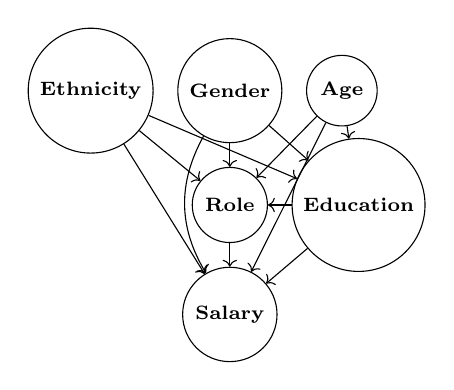
\begin{tikzpicture}[node distance=0.6cm and 1cm, every node/.style={minimum size=0.5cm}]
        \tikzset{vertex/.style = {draw, circle, align=center}}

        \node[vertex] (Ethnicity) {\bf\scriptsize{{Ethnicity}}};
        \node[vertex, right=0.3cm of Ethnicity] (Gender) {\bf{\scriptsize{Gender}}};
        \node[vertex, right=0.3cm of Gender] (Age) {\bf{\scriptsize{Age}}};
        \node[vertex, below=0.3cm of Gender] (Role) {\bf{\scriptsize{Role}}};
        \node[vertex, right=0.3cm of Role] (Education) {\bf{\small{\scriptsize{Education}}}};
        \node[vertex, below=0.3cm of Role] (Salary) {\bf{\scriptsize{Salary}}};

        \draw[->] (Ethnicity) -- (Salary);
        \draw[->] (Gender) -- (Role);
        \draw[->] (Age) -- (Role);
         \draw[->] (Education) -- (Role);
           \draw[->] (Education) -- (Salary);
             \draw[->] (Ethnicity) -- (Education);
                \draw[->] (Ethnicity) -- (Role);
             \draw[->] (Gender) -- (Education);
               \draw[->] (Age) -- (Education);
                 \draw[->] (Role) -- (Salary);
        \draw[->] (Gender) to[bend right] (Salary);
        \draw[->] (Age) -- (Salary);
    \end{tikzpicture}
    \caption{Partial causal DAG for the Stack Overflow dataset.}
    \label{fig:causal_DAG}
\end{figure}



 \begin{example}
Figure \ref{fig:causal_DAG} depicts a partial causal DAG for the SO dataset over the attributes in Table \ref{tab:data} as endogenous variables (we use a larger causal DAG with all 20 attributes in our experiments). 
  Given this causal DAG, we can observe that the role that a coder has in their company depends on their education, age gender and ethnicity.
\end{example}
\par


\par
\paratitle{Intervention} In Pearl's model, a treatment $T = t$ (on one or more variables) is considered as an {\em intervention} to a causal DAG by mechanically changing the DAG such that the values of node(s) of $T$ in $G$ are set to the value(s) in $t$, which is denoted by $\doop(T = t)$. Following this operation, the probability distribution of the nodes in the graph changes as the treatment nodes no longer depend on the values of their parents. Pearl's model gives an approach to estimate the new probability distribution by identifying the confounding factors $Z$ described earlier using conditions such as {\em d-separation} and {\em backdoor criteria} \cite{pearl2009causal}, which we do not discuss in this paper.


\par
\paratitle{Average Treatment Effect} The effects of an intervention are often measured by evaluating
% \par
% \paratitle{Causal inference, Treatment, ATE, and CATE}
% \newtextold{One of the primary goals  of {\em causal inference} is to estimate the effect of making a change in terms of a {\em treatment} $T$ (often referred to as an intervention)
% on the outcome $O$. 
% %A variable that is modified is often referred to as the treatment variable $T$ and the metric used to captures 
% The effect of treatment $T$ on outcome $O$ is measured by 
% %is known as 
{\em Conditional Average treatment effect (CATE)}, 
%a {\em treatment variable} $T$ on an outcome variable $O$ (e.g., what is the effect of higher \verb|Education| on \verb|Salary|). 
measuring the effect of an intervention on a subset of records~\cite{rubin1971use,holland1986statistics} by calculating the difference in average outcomes between the group that receives the treatment and the group that does not (called the {\em control} group), providing an estimate of how the intervention by $T$ influences an outcome $O$ for a given subpopulation. 
% Mathematically,
% \begin{equation}
%     %{\small ATE(T,O) = \mathbb{E}[O \mid \doop(T=1)] -      \mathbb{E}[O \mid \doop(T=0)]}
%     {\small ATE(T, O) = \mathbb{E}[O \mid \doop(T=1)] -  
%     \mathbb{E}[O \mid \doop(T=0)]}
% \label{eq:ate}
% \end{equation}
% In our work, where the treatment with maximum effect may vary among different subpopulations, we are interested in computing the \emph{Conditional Average Treatment Effect} (CATE), which measures the effect of a treatment on an outcome on \emph{a subset of input units}~\cite{rubin1971use,holland1986statistics}. 
Given a subset of the records defined by (a vector of) attributes $B$ and their values $b$, 
%g {\in} \Qagg(\db)$ defined by a predicate $G {=} g$ 
we can compute $CATE(T,O \mid B = b)$ as:
{
\begin{eqnarray}    
    %CATE(T,O \mid G=g) = \mathbb{E}[O \mid \doop(T=1)&, G=g] -  \mathbb{E}[O \mid \doop(T=0), G=g] 
   % CATE(T,O \mid B = b) = 
    \mathbb{E}[O \mid \doop(T=1), B = b] -  
    \mathbb{E}[O \mid \doop(T=0), B = b]\label{eq:cate}
\end{eqnarray}
}
Setting $B=\phi$ is equivalent to the ATE estimate.
The above definitions assumes that the treatment assigned to one unit does not affect the outcome of another unit (called the {Stable Unit Treatment Value Assumption (SUTVA)) \cite{rubin2005causal}}\footnote{This assumption does not hold for causal inference on multiple tables and even on a single table where tuples depend on each other.}. 


The ideal way of estimating the ATE and CATE is through {\em randomized controlled experiments}, 
where the population is randomly divided into two groups (treated and control, for binary treatments): 
%treated group that receives the treatment and control group that does not (denoted by 
%{the \em treated} group 
denoted by 
$\doop(T = 1)$ 
%for a binary treatment)  (the {\em control} group, 
and $\doop(T = 0)$ resp.)~\cite{pearl2009causal}.
%\sr{edited up to here, going to read the rest first, this section should not look like causumx}
%\par
%\par
However, randomized experiments cannot always be performed due to ethical or feasibility issues. In these scenarios, observational data is used to estimate the treatment effect, which requires the following additional assumptions. 
% {\em Observational Causal Analysis} still allows sound causal inference under additional assumptions. Randomization in controlled trials mitigates the effect of {\em confounding factors}, i.e., attributes that can affect the treatment assignment and outcome. Suppose we want to understand the causal effect of \verb|Education| on \verb|Salary| from the SO dataset.  %in Example~\ref{ex:running_example}. 
% We no longer apply Eq. (\ref{eq:ate}) since the values of \verb|Education| were not assigned at random in this data, and obtaining higher education largely depends on other attributes like \verb|Gender|, \verb|Age|, and \verb|Country|. 
% Pearl's model provides ways to account for these confounding attributes $Z$ to get an unbiased causal estimate from observational data under the following assumptions ($\independent$ denotes independence):
% \vspace{-2mm}
\newtextold{
The first assumption is called {\em unconfoundedness} or {\em strong ignorability}  \cite{rosenbaum1983central} says that the independence of outcome $O$ and treatment $T$ conditioning on a set of confounder variables  (covariates) $Z$, i.e.,
%\begin{eqnarray}
 $    O \independent T | Z {=} z$.
 %\label{eq:unconfoundedness}
%\end{eqnarray}
The second assumption called {\em overlap or positivity} says that there is a chance of observing individuals in both the treatment and control groups for every combination of covariate values, i.e., 
%\begin{eqnarray}
   $ 0 < Pr(T {=} 1 ~~|~~Z {=} z)< 1 $.
   %\label{eq:overlap}
%\end{eqnarray}
}
%\sg{Is this overlap or positivity? maybe both are the same?} \sr{yeah - same - from Google AI - The overlap assumption, also known as the positivity assumption, is a key assumption in causal inference that states that there is a chance of observing individuals in both the treatment and control groups for every combination of covariate values.}
% The above conditions are known as {\em Strong Ignorability} in Rubin's model \cite{rubin2005causal}.
The unconfoundedness assumption requires that the treatment $T$ and the outcome $O$ be independent when conditioned on a set of variables $Z$. In SO, assuming that only $Z$ =\{\verb|Gender|, \verb|Age|, \verb|Country|\} affects $T = $ \verb|Education|, if we condition on a fixed set of values of $Z$, i.e., consider people of a given gender, from a given country, and at a given age, then $T = $ \verb|Education| and $O = $ \verb|Salary| are independent. For such confounding factors $Z$,  Eq. (\ref{eq:cate}) reduces to the following form 
(positivity 
gives the feasibility of the expectation difference): 
 \vspace{-1mm}
{\small
\begin{flalign}    
% \begin{eqnarray}
   % % & ATE(T,O) = \mathbb{E}_Z \left[\mathbb{E}[O \mid T=1, Z = z] -  
   %  \mathbb{E}[O \mid T=0, Z = z] \right] \label{eq:conf-ate}\\
 & CATE(T,O {\mid} B {=} b) {=} \nonumber
    \mathbb{E}_Z \left[\mathbb{E}[O {\mid} T{=}1, B {=} b, Z {=} z] {-}  
    \mathbb{E}[O {\mid} T{=}0, B {=} b, Z {=} z]\right]\label{eq:conf-cate}
\end{flalign}
% \end{eqnarray}
}
% \vspace{-4mm}
This equation contains conditional probabilities and not $\doop(T = b)$, which can be estimated from an observed data. 
Pearl's model gives a systematic way to find such a $Z$ when a causal DAG is available. 




\section{Design Overview \label{design}} 
%
\subsection{System Model}
\noindent {\bf Network:}
We assume a single verifier (\vrf) and a network of multiple low-end embedded devices as 
\prv-s. \vrf is assumed to be trusted and sufficiently powerful. 
The network is assumed to be: (1) connected, i.e., there is always a path between \vrf and any of  
\prv-s, and (2) quasi-static during attestation, i.e., its topology can change as long as the changes 
do not influence the path of message propagation. \system is network-agnostic and can be 
realized over any popular medium (e.g., WiFi, Bluetooth, Cellular, Zigbee, Matter).

\noindent {\bf $\boldsymbol{\ra}$ Architecture in $\boldsymbol{\prv}$:}
All \prv-s must support \rata or \casu architecture: in a given deployment, either all support
the former or all support the latter, i.e., no mixing.\footnote{This is not a hard requirement,
meaning that a mix of \rata and \casu devices would work as well;
however, it makes the presentation simpler.}
As mentioned in Section \ref{sec:bg}, an attestation token in 
\rata is computed as a keyed hash over a small fixed-size input.

In contrast, \casu prevents any PMEM modification (except via secure update), 
thus obviating the entire need for \ra. However, \casu does not offer \prv liveness.
Note that, in any secure \ra technique, an attestation token returned by \prv 
provides both attestation and \prv liveness.
The latter is important for detecting whether \prv is operational, i.e., not powered off, 
destroyed/damaged, or physically removed. 
To this end, \casu supports a ``secure heartbeat'' feature, whereby 
\vrf periodically issues a random challenge and \prv simply computes (and returns) a keyed 
hash over that challenge. This costs about the same as attestation token computation in \rata. 
We discuss various use-cases of \rata and \casu in Section \ref{subsec:rata-casu-comparison}.

\noindent {\bf Network Interface in $\boldsymbol{\prv}$:}
The primary network interface of each \prv is placed within \system's Trusted Computing Base (TCB). 
This ensures that \system protocol messages are handled with the highest 
priority, even in the presence of malware or run-time attacks.
\system uses two special attestation-specific packet types: request and report. 
Normal software outside TCB is prevented from sending or receiving these packet types;
this is achieved by inspecting each incoming/outgoing packet header
in order to prevent tampering with, and forgery of, \system messages. Furthermore, 
\system packets are always handled with higher priority than other tasks. 
This approach is based on NetTCB of \garota \cite{garota}.
Besides, we adopt TimerTCB from \garota to guarantee (nearly) synchronized attestation start times.

With these security features, \rata-enabled \prv-s are safeguarded against
full compromise and malware-based disruption of the attestation process.
The benefit is more subtle in the case of \casu: although \casu guarantees no malware,
software running on \casu-enabled \prv-s can still be susceptible to control-flow attacks, 
which would prevent, or delay, receiving of \vrf attestation requests and 
generation of secure heartbeats. The above features ensure that this does not occur.

\noindent {\bf $\boldsymbol{\prv}$ TCB:}
\system TCB includes both hardware and software components, i.e., akin to \rata and \casu, 
\system is a {\bf hybrid} architecture. In addition to the trusted software of either \rata or \casu, 
\system software includes TimerTCB, NetTCB, and \sa logic described in Section \ref{sec:protocol}.
The primary network interface (NetTCB) is shared between the \system software  
and other non-TCB software. Incoming messages cause an interrupt via NetTCB.
\system software prioritizes \system protocol messages. It forwards other incoming messages to the intended
application (outside TCB) and outgoing messages to the destination.
TCB hardware components are:
%
\begin{compactitem}
    \item NetTCB -- Network interface for \system messages
    \item TimerTCB -- Timer used for simultaneous attestation
    \item DMEM segment reserved for running \system software 
    \item Part of ROM reserved for \system software, key shared with \vrf, and hash chain data
\end{compactitem}
\subsection{Adversary Model \label{sec: adversary}}
%
In line with other network attestation (\sa) techniques, \system considers software-only 
remote network attacks. We assume an adversary (\sadv) that can inject malware and exercise 
full control over a compromised \prv, except for its TCB. \sadv can manipulate any non-TCB
peripherals and external components, such as Direct Memory Access (DMA), sensors, actuators, 
and other (non-primary) network interfaces. Also, \sadv has comprehensive knowledge 
of software (i.e., non-\system software) running on \prv,
including its memory vulnerabilities. Thus, it can launch run-time (e.g., control-flow) attacks.

We also consider a network-based \sadv represented by a malicious (non-\system) entity in the
\prv network. Consequently, all packets exchanged between \vrf and \prv-s can 
be manipulated by \sadv: based on the Dolev-Yao model \cite{dolevYao}, \sadv can eavesdrop on, 
drop, delay, replay, modify, or generate any number of messages. 

\noindent {\bf DoS Attacks:}
\system prevents DoS attacks that attempt to ``brick'' \prv-s via malware,
or control-flow attacks. However, DoS attacks that jam the network or attempt to inundate 
specific \prv's network interfaces are out of scope. 
For countermeasures, we refer to well-known techniques, 
such as \cite{muraleedharan2006jamming,zhijun2020low, mamdouh2018securing}.

\noindent {\bf Physical Attacks:}
\system does not offer protection against physical attacks, both 
invasive (e.g., via hardware faults and reprogramming through debuggers) and non-invasive (e.g., 
extracting secrets via side-channels). Such attacks can be mitigated, at considerable cost, via
well-known tamper-resistance methods \cite{obermaier2018past,ravi2004tamper}.

\subsection{Protocol Elements \label{elems}}
%
As mentioned in Section \ref{intro}, we construct two \system variants, 
based on the availability of a real-time clock (RTC) on \prv-s:
%
\begin{compactenum}[(1)]
    \item \textbf{$\boldsymbol{\trapsrtc}$:} Each \prv has an RTC. In an attestation request, \vrf includes 
    the exact time when all \prv-s should perform attestation. 
    \item \textbf{$\boldsymbol{\trapsnortc}$:} \prv-s do not have RTC-s. In an attestation request, 
    \vrf provides the height of the spanning tree, composed of all \prv-s. Each \prv 
    estimates the time to perform attestation using spanning tree height and its own secure timer.
\end{compactenum}

\noindent \trapsrtc is designed for an ideal best-case scenario where each \prv is assumed to 
have a synchronized RTC. \toctousa window is completely removed in \trapsrtc.
On the other hand, \trapsnortc is intended for a more realistic scenario where each \prv has a timer.
Although \trapsnortc can not offer precisely synchronized attestations on \prv-s, it still significantly reduces \toctousa. Section \ref{subsec:security-analysis} provides further details.

\noindent{\bf $\boldsymbol{\toctousa}$ resilience}
Due to the availability of RTC in \trapsrtc and the spanning tree's height in \trapsnortc, 
all \prv-s perform attestation almost simultaneously. Figure \ref{fig: toctou window}(b) 
shows the eliminated \toctou window in \trapsrtc.

\noindent {\bf Attestation Regions:}
Unlike prior \sa schemes which perform attestation over the 
entire PMEM, \system is built on top of either \rata or \casu, which enables \prv to 
compute a MAC over a short fixed size including:
(1) \lmt\ and \vrf's challenge, in \rata,  or (2) merely \vrf's challenge, in \casu.
Section \ref{sec:protocol} provides details about other parameters included in the MAC computation.

\noindent {\bf Authentication of Attestation Requests:}
Most prior work in network (or swarm) attestation
does not take into account authentication of attestation requests. While this may or may
not be an issue in a single \prv{} \ra setting\footnote{\vrf authentication in a single \prv 
setting is thoroughly discussed in \cite{Brasser-DAC16}.}, it certainly becomes a concern in \sa.
If requests are not authenticated, \sadv can readily mount a DoS attack whereby \sadv floods all 
\prv-s with bogus requests, each of which causes {\bf all} \prv-s to perform attestation and 
generate numerous useless replies.

This issue is deceptively simple. The na\"ive approach to address the problem is for \vrf
(which already shares a unique symmetric key with each \prv) to send 
an individual attestation request to every \prv, authenticated with each shared key.
This is unscalable for obvious reasons. 

Another intuitive approach is to assume that every \prv knows \vrf's
public key and \vrf simply signs each attestation request with a timestamp. Despite scaling well, this 
approach opens the door for a simple DoS attack whereby \sadv floods the network with 
attestation requests with fake signatures, forcing all \prv-s to verify them, and due to failed
verification, discard the requests. This incurs heavy collective computational 
overhead on the entire network.

Yet another trivial method is to assume a separate group key (shared among \vrf and all \prv-s) that is
used exclusively for authenticating \vrf-issued attestation requests. This is quite efficient
since a simple MAC (realized as a keyed hash) would suffice. However, a key shared among a potentially
large number of \prv-s raises the risk of its eventual compromise, which would have 
unpleasant consequences. 
Also, managing the group and key revocation becomes increasingly complex as the network grows.

\system uses hash chains to authenticate attestation requests. Hash chains, as described in Section 
\ref{chains}, are well-known constructs used in numerous similar settings where symmetric keys 
are unscalable and traditional public key signatures are too expensive.
They provide forward security and efficient verification, while offering relatively simple
key management. Although hash chains suffer from some fragility in terms of synchronization 
and timing requirements, these issues are more palatable than those that stem from managing 
large numbers of shared keys.


\section{\system Protocols} \label{sec:protocol}
%
This section describes two protocol variants.
The notation used in the rest of the paper is summarized in Table \ref{table:notation}.

\noindent{\bf Assumptions:}
As mentioned above, we assume that each \prv shares a unique symmetric key (\key) with \vrf. 
Also, throughout a single attestation instance, \vrf is assumed to be within the broadcast range 
of at least one \prv, and the entire \prv network must remain connected during this time.
Furthermore, all \prv-s have a parameter (\maxdelay) that denotes the maximum attestation report (\Attrep)
propagation delay in the network. In the absolute worst case of a line topology, it can
be set as: $\maxdelay=n*t_{report}$, where $n$ is the number of \prv-s and $t_{report}$ is the \Attrep\ propagation delay.
We also assume that the attestation request (\Attreq) propagation delay ($t_{request}$) 
and the \Attreq\ verification time ($t_{hash}$) are known to all \prv-s.
\maxdelay\ is needed to limit the time when 
each \prv forwards other \prv-s' attestation results towards \vrf.
For the sake of simplicity, we assume that no new attestation requests 
are issued while one is being served.

\noindent {\it NOTE:} As mentioned at the end of Section \ref{elems}, the use of hash 
chains for \vrf authentication is optional; a separate group key shared between \vrf and all \prv-s 
could be used instead, albeit with the risk of its possible leak.

\subsection{\trapsrtc: RTC-Based \sa Technique}\label{sec:one}
%
Commodity RTCs, such as MCP7940MT-I/SM \cite{rtc}, are now readily available for 
under $\$0.60$ per unit. This affordability marks a significant shift from the past, 
when real-time security features were often too costly for IoT devices. This motivates 
our design of an \sa protocol for devices with RTCs.
We begin by presenting this simple variant of the core ideas of \system.
An alternative variant without the RTC requirement is described in Section \ref{sec:two}.
\trapsrtc pseudo-code is shown in Algorithms \ref{alg:rtc_prv} and \ref{alg:rtc_vrf}.


%
\begin{figure}
    \centering
    \includegraphics[height=1.2in,width=0.7\columnwidth]{images/vrf_FSM.pdf}
    \vspace{-.5em}
    \caption{\vrf\ State Machine}
    \label{fig:vrfFSM}
    \vspace{-1.5em}
\end{figure}
%
\begin{compactitem}[]
    \item {\bf \underline{\bf V1.} Idle:} \vrf waits for an external signal to begin an attestation instance. 
    When it occurs, \vrf transitions to \textbf{Initiate}.
    %
    \item {\bf \underline{\bf V2.} Initiate:} \vrf assigns \attesttime{}, 
    %
    as described in Section \ref{section:timeout}, which accounts for request 
    propagation and network height. (\attesttime{} is computed by each \prv in \trapsnortc.)     
    %
    It then initializes 
    \textit{Attest}=\textit{Fail}=$\emptyset$, and \textit{NoRep}=\{\devid-s of all \prv-s\}. 
    Next, \vrf sets \snd\ to \vrf, composes \Attreq, and broadcasts it. (Recall the assumption 
    that at least one \prv must be within broadcast range of \vrf at this time.) 
    It then sets a local timer to \timeout{},
    %
    as detailed in Section \ref{section:timeout}, which factors into network size and delays, 
    %
    and then transitions to \textbf{Collect}.
    %
    \item {\bf \underline{\bf V3.} Collect:} \vrf waits for \Attrep-s. 
    Upon receipt of an \Attrep, \vrf first checks that \hash\ contained in \Attrep\ matches that in the 
    currently pending \Attreq; otherwise, it is discarded. Next, \vrf validates \Attrep\ by 
    looking up the corresponding \key shared with \prv (identified by \devid) and recomputing 
    the MAC. If MAC validation fails, \Attrep\ is discarded. Otherwise:
    \begin{compactitem}[]
        \item {\it \underline{V3.1}} (\casu): \devid\ is moved from \textit{NoRep} to \textit{Attest}.
        \item {\it \underline{V3.2}} (\rata): \vrf maintains the last valid \lmt\ for each \prv. 
    When processing an \Attrep\ from a given \prv, \vrf compares received \lmt$'$\ with the stored 
    \lmt\ for that \prv. A mismatch signifies failed attestation and
    \devid\ is added to \textit{Fail}. Otherwise, it is added to \textit{Attest}. 
    In either case, \devid\ is removed from \textit{NoRep}.
        \item {\it \underline{V3.3}} If $\textit{NoRep}=\emptyset$, \vrf transitions to \textbf{Tally}.
        \item {\it \underline{V3.4}} If \timeout\ timer expires, \vrf transitions to \textbf{Tally}.
    \end{compactitem}
    \item {\bf \underline{\bf V4.} Tally:} \vrf outputs \textit{Attest}, \textit{Fail}, and 
    \textit{NoRep}. It then returns to \textbf{Idle}.
    %
\end{compactitem}


\begin{algorithm}[hbt!]
\footnotesize
\caption{Pseudo-code of $\boldsymbol{\trapsrtc}$ for \prv}\label{alg:rtc_prv}
    \begin{algorithmic}[1]
    \While{True}
        \State \textit{m} = RECEIVE()
        \If {TYPE(\textit{m}) == \textit{``req''}}
            \State [\snd, \hashind, \hash, \attesttime] $\gets$ DECOMPOSE(\textit{m})
            \If {$\curhashind <= \hashind$}
                \State CONTINUE() 
            \EndIf
            \If {GET\_TIME() $>=$ \attesttime}
                \State CONTINUE() 
            \EndIf
            \If {\textit{H}$^{(\curhashind-\hashind)}(\hash)$ $\neq$ \curhash}
                \State CONTINUE()
            \EndIf
             \State \parent $\gets$ \snd; \curhashind $\gets$ \hashind; \curhash $\gets$ \hash; \textit{attestTime} $\gets$ \attesttime;
             \State BROADCAST(\textit{``req''}, \devid, \curhashind, \curhash, \attesttime)
             \State \textit{CurTime} $\gets$ \textit{GET\_TIME()} \Comment{Get current time from RTC}
             \While {\textit{CurTime} $<$ \attesttime} \Comment{non-busy-waiting}
             \State \textit{CurTime} $\gets$ GET\_TIME()
        % %%%%%
             \EndWhile
             \State \attesttime$'$ $\gets$ \textit{CurTime}
             \State \Authrep $\gets$ MAC(\key, \parent, \attesttime$'$, \hash, \{\lmt\})
             \State \Attrep $\gets$ \textit{``rep''}, \devid, \parent, \attesttime$'$,  \hash, \{\lmt\}, \Authrep
             \State UNICAST(\parent, \Attrep)
             \State SET\_TIMER(\height*t$_{report}$)
        \EndIf
         \If {TYPE(\textit{m}) == \textit{``rep''}}
                 \If {\hash == GET\_\hash(\textit{m})}
                     \State UNICAST(\parent, \textit{m})
                 \EndIf
        \EndIf
    \EndWhile
    \end{algorithmic}
\end{algorithm}


\begin{algorithm}[hbt!]
\footnotesize
\caption{Pseudo-code of $\boldsymbol{\trapsrtc}$ for \vrf}\label{alg:rtc_vrf}
    \begin{algorithmic}[1]
    \While{True}
        \State \textit{type} $\gets$ REQUEST\_TYPE() 
        \State \hashind $\gets$ GET\_HASH\_IND()
        \State \hash $\gets$ GET\_HASH(\hashind)
        \State \attesttime $\gets$ \netheight*(t$_{request}$+t$_{hash}$)+t$_{slack}$+\textit{GET\_TIME()}
        \State \Attreq $\gets$ \textit{``req'', vrf}, \hashind, \hash, \attesttime
        \State \textit{Attest} $\gets \emptyset$; \textit{Fail} $\gets \emptyset$; \textit{NoRep} $\gets$ \{\devid-s of all \prv-s\}
        \State BROADCAST(\Attreq)
        \State T $\gets$ GET\_TIME()
        \While{\attesttime $<$ T $<$ \timeout}
             \State \Attrep $\gets$ RECEIVE()
             \State [\devid, \parent, \attesttime, \hash, \lmt, \Authrep] $\gets$ DECOMPOSE(\textit{\textit{m}})
             \State \lmt$'$ $\gets$ LMT\_LIST(\devid) \Comment{\casu skips \#13, \#15, \#17, \#18}
             \If{(\hash \ == \curhash) \ AND 
             (MAC(\key, \parent, \attesttime, \hash, \{\lmt\}) == \Authrep)}
                 \If {\lmt == \lmt$'$} 
                     \State \textit{Attest} $\gets$ \textit{Attest} $\cup$ \devid
                 \Else
                     \State \textit{Fail} $\gets$ \textit{Fail} $\cup$ \devid
                 \EndIf
             \State \textit{NoRep} $\gets$ \textit{NoRep} $\backslash$ \devid
             \EndIf
        \EndWhile
        \State OUTPUT(\textit{Attest}, \textit{Fail}, \textit{NoRep})
    \EndWhile
    \end{algorithmic}
\end{algorithm} 

\trapsrtc\ has two message types:

\noindent \textbf{Attestation Request ($\boldsymbol{\Attreq}$):} Generated by \vrf, 
it contains: \hash, \hashind, and \attesttime, which are used to authenticate \Attreq. Note that \hash\ 
is used as a challenge for this \sa. $\boldsymbol{\Attreq}$ also includes
the packet type field: \textit{``req''} and the identifier \snd\ of either \vrf 
that originated it (for the first hop), or a \prv that forwards it (for subsequent hops).
\snd\ is used by each receiving \prv to learn its parent in the spanning tree.

\noindent \textbf{Attestation Report ($\boldsymbol{\Attrep}$):} Generated by each \prv, this 
message carries the attestation report. It contains an authentication token (\Authrep), which provides message integrity. 
\lmt$'$\ is included in the calculation of \Authrep\ and in \Attrep\ only for \rata-enabled \prv-s. 
Similar to $\boldsymbol{\Attreq}$, $\boldsymbol{\Attrep}$
also includes the packet type field: \textit{``rep''}  and the identifier of \prv that generated 
this report. Also, \Attrep\ includes \hash\ that was received in \Attreq\ and the actual time 
(\attesttime$'$) when attestation is performed.

\begin{table}[ht]
    \vspace{.7em}
    \footnotesize
    % \scriptsize
    \begin{tabularx}{\linewidth}{|c|X|}
        \hline
        \rowcolor{gray!20}
        {\bf Notation} & \multicolumn{1}{c|}{\bf Meaning} \\            
        \thickhline
        $\devid$ & Identifier of responding $\prv$ \\
        \hline
        $\parent$ & Identifier of responding $\prv$'s parent \\
        \hline
        $\snd$ & Identifier of the sending device \\
        \hline
        $H()$ & Cryptographic hash function (e.g., SHA2-256) used in hash chain computation \\
        \hline 
        $H^s(x)$ & Denotes $s>1$ repeated applications of $H()$ starting with initial input $x$ \\
        \hline        
        $\hash$ & Hash value sent by $\vrf$ that authenticates it to all $\prv$-s; 
            it also serves as the challenge for this $\sa$ instance \\
        \hline
        $\curhash$ & Current hash value stored by $\prv$ \\
        \hline
        $\hashind$ & Index of $\hash$ sent by $\vrf$  \\
        \hline
        $\curhashind$ & Index of $\curhash$ stored by $\prv$ \\
        \hline
        $\netheight$ & Network spanning tree height  \\
        \hline
        $\height$ & Height of $\prv$ in the spanning tree \\
        \hline        
        $\lmt$ & Last Modification Time (of PMEM), only used in $\rata$, stored on \vrf \\        
        \hline
        $\lmt'$ & Last Modification Time (of PMEM), only used in $\rata$, stored on \prv \\        
        \hline
        \key & Shared key between \prv and \vrf, securely stored on \prv and restricted to its trusted attestation code \\
        \hline
        $\Attreq$ & \parbox[c]{1\linewidth}{\vspace{2pt}\raggedright Attestation request message ($\vrf \rightarrow \prv$): \\
        \phantom{}[\textit{"req"}, \snd, \hash, \hashind, \attesttime]}\vspace{1pt}\\
\hline
        $\Attrep$ & \parbox[c]{1\linewidth}{\vspace{2pt}\raggedright Attestation report message ($\vrf \leftarrow \prv$): \\
        \phantom{}\tiny{[\textit{"rep"}, \devid, \parent, \attesttime$'$, \hash, \{\lmt\}, \Authrep]}}\vspace{1pt}\\
\hline
        $\Authrep$ & \parbox[c]{1\linewidth}{\vspace{2pt}\raggedright 
           Authentication of attestation report in $\Attrep$: \\ 
           \tiny{MAC(\key, \parent, \attesttime$'$, \hash, \{\lmt$'$\})}}\vspace{1pt}\\
        \hline
        t$_{request}$ & propagation delay of $\Attreq$\\
        \hline
        t$_{report}$ & propagation delay of $\Attrep$\\
        \hline
        t$_{hash}$ & Computation time for $\Attreq$ verification \\
        \hline        
        t$_{MAC}$ & Computation time for MAC generation \\
        \hline
        t$_{slack}$ & Additional slack time \\
        \hline
        $\maxdelay$ & Max delay to receive an $\Attrep$ from a descendant $\prv$ \\
        \hline
        $\attesttime$ & Time to begin attestation, set by $\vrf$ \\
        \hline        
        $\attesttime'$ & Time when a given $\prv$ actually performed attestation \\
        \hline
        $\timeout$ & $\vrf$'s timeout for receiving all attestation replies \\
        \hline
    \end{tabularx} 
    \caption{Notation Summary} 
    \vspace{-3em}
    \label{table:notation}
\end{table}

We now describe \prv operation as a state machine with five states, as shown in 
Figure \ref{fig:prvFSM}: {\it Idle, Verify, Attest-Wait, Attest,}  and {\it Forward-Wait}.

\begin{figure}
    \centering
    \includegraphics[height=1.5in,width=0.7\columnwidth]{images/prv_FSM.pdf}
    \vspace{-1em}
    \caption{\prv\ State Machine} 
    \label{fig:prvFSM}
    % \vspace{-2em}
\end{figure}
%

\begin{compactitem}[]
%
    \item {\bf \underline{\bf P1.} Idle:} \prv runs normally. Upon receiving an \Attreq, it 
    proceeds to \textbf{Verify}. Any \Attrep\ received in this state is discarded.
%
    \item {\bf \underline{\bf P2.} Verify:} 
    \begin{compactitem}[]
        \item \underline{\it P2.1:} \prv checks if $\curhashind>\hashind$ and $\attesttime>T$,
    where $T$ is its current RTC value. If either check fails, it discards \Attreq\ and 
    returns to {\bf Idle}. 
        \item \underline{\it P2.2:} \prv computes and checks whether $H^s(\hash) \stackrel{?}{=} 
    \curhash$, where $s=\curhashind-\hashind$.\footnote{Recall that it is possible for $s>1$,
    (as discussed at the end of Section \ref{chains}) meaning that \prv became de-synchronized.
    Also, \hashind\ is decremented by one in every \ra instance.}
    If not, it discards \Attreq\ and returns to {\bf Idle}.
    (Note that a \prv might receive duplicate \Attreq-s from multiple neighbors; it simply discards them.)
    \item \underline{\it P2.3:} \prv\ replaces: \curhash\ with \hash, and \curhashind\ with \hashind. 
    Then, \prv stores \snd\ as \parent, sets \snd\ field of received \Attreq\ to its \devid, and 
    broadcasts modified \Attreq.
    %\vspace{.1cm}
    \item \underline{\it P2.4:} \prv sets (using its RTC) a secure timer (TimerTCB) to \attesttime\ 
    and transitions to \textbf{Attest-Wait}.
    \end{compactitem} 
%
     \item {\bf \underline{\bf P3.} Attest-Wait:} \prv runs normally while the timer is ticking. 
     If any \Attreq\ is received in this state, it is discarded. 
%
    \item {\bf \underline{\bf P4.} Attest:} When the timer matches \attesttime, \prv sets {\it \attesttime$'$} 
    to the current RTC value, computes \Authrep{}, and composes 
    \Attrep\ as defined above. It then uni-casts \Attrep\ to \parent{}, sets the timer 
    to \maxdelay, and transitions to \textbf{Forward-Wait}.
%    
% \vspace{0.2cm}
    \item {\bf \underline{\bf P5.} Forward-Wait:} \prv runs normally while the timer is ticking. If \prv 
    receives an \Attrep, it checks whether the report's \hash\ matches that previously received 
    in \textbf{Verify}. If not, it is discarded. Otherwise, \prv uni-casts received \Attrep\  
    to its parent and remains in \textbf{Forward-Wait}. When the timer matches \maxdelay, \prv transitions 
    to \textbf{Idle}. Note that any \Attreq \ received while in this state 
    is discarded. 
%
\end{compactitem}

Whereas, as shown in Figure \ref{fig:vrfFSM}, \vrf's state machine has four states: 
{\it Idle, Initiate, Collect,} and {\it Tally}.



\subsection{\trapsnortc: Clockless \sa Technique}\label{sec:two}

Despite its relatively low cost, an RTC might still not be viable for some IoT deployments. 
This leads us to construct a \system variant without RTCs.
Pseudo-code for \trapsnortc is shown in Algorithms \ref{alg:nortc_prv} and \ref{alg:nortc_vrf}.

\begin{algorithm}[hbt!]
\footnotesize
 \caption{Pseudo-code of $\boldsymbol{\trapsnortc}$ for \prv}\label{alg:nortc_prv}
     \begin{algorithmic}[1]
     \While{ True }
         \State \textit{m} = RECEIVE()
         \If {TYPE(\textit{m}) == ``req''}
             \State [\snd, \hashind, \hash, \height, \netheight, \attesttime] $\gets$ DECOMPOSE(\textit{m})
             \If {$\curhashind <= \hashind$}
                 \State CONTINUE() 
             \EndIf
             
             \If {\textit{H}$^{(\curhashind-\hashind)}$(\hash) $\neq$ \curhash}
                 \State CONTINUE()
             \EndIf
             \State \parent $\gets$ \snd; \curhashind $\gets$ \hashind; \curhash $\gets$ \hash; \textit{attestTime} $\gets$ \attesttime;
             \State BROADCAST(\textit{``req''}, \devid, \curhashind, \curhash, \height + 1, \netheight, \attesttime)
        
             \State \textit{timer} $\gets$ \textit{startTimer()} \Comment{start a timer}
             \State \textit{attestWait} $\gets$ (\netheight-\height)*(\textit{t$_{request}$+\textit{t$_{hash}$})}
        
             \While {\textit{timer} $<$ \textit{attestWait}} \Comment{non-busy-waiting}%do something here
                 \State WAIT()
             \EndWhile
             \state \attesttime$'$ $\gets$ \textit{timer}
             \State \Authrep $\gets$ MAC(\key, \parent, \attesttime, \hash, {\lmt})
             \State \Attrep $\gets$ \textit{``rep''}, \devid, \parent, \attesttime$'$, \hash, {\lmt}, \Authrep
             \State UNICAST(\parent, \Attrep)
             \State SET\_TIMER(\height*\textit{t$_{report}$})
         \EndIf
         \If {TYPE(\textit{m}) == \textit{``rep''}}
                 \If {\hash == GET\_\hash(\textit{m})}
                     \State UNICAST(\parent, \textit{m})
                \EndIf
        \EndIf
    \EndWhile
     \end{algorithmic}
 \end{algorithm}

 
 \begin{algorithm}[hbt!]
\footnotesize
 \caption{Pseudo-code of $\boldsymbol{\trapsnortc}$ for \vrf}\label{alg:nortc_vrf}
     \begin{algorithmic}[1]
     \While{True}
         \State \textit{type} $\gets$ REQUEST\_TYPE() 
         \State \hashind $\gets$ GET\_HASH\_IND()
         \State \hash $\gets$ GET\_HASH(\hashind)
         \State \attesttime $\gets$ \textit{\netheight}*(t$_{request}$+$t_{hash})+t_{slack}$+\textit{GET\_TIME()}
         \State \netheight $\gets$ GET\_NET\_height()
    
         \State \Attreq $\gets$ \textit{``req''}, \vrf, \hashind, \hash, 0, \netheight, \attesttime
         \State Attest $\gets \emptyset$; Fail $\gets \emptyset$; NoRep $\gets$ \{\devid-s of all \prv-s\}
         \State BROADCAST(\textit{InitID}, \Attreq)
         \State T $\gets$ GET\_TIME()
        \While{T $<$ \timeout}
             \State \Attrep $\gets$ RECEIVE()
             \State [\devid, \parent, \attesttime, \hash, \{\lmt\}, \Authrep] $\gets$ DECOMPOSE(\textit{\textit{m}})
             \State \lmt$'$ $\gets$ LMT\_LIST(\devid) \Comment{\casu skips \#14, \#16, \#18, \#19}
             \If{(\hash \ == \curhash) \ AND  (MAC(\key, \parent, \attesttime, \hash, \{\lmt\}) == \Authrep)}
                 \If {\lmt == \lmt$'$}
                     \State \textit{Attest} $\gets$ \textit{Attest} $\cup$ \{\devid\}
                 \Else
                     \State \textit{Fail} $\gets$ \textit{Fail} $\cup$ \{\devid\}
                 \EndIf
             \State \textit{NoRep} $\gets$ \textit{NoRep} $\backslash$ \{\devid\}
             \EndIf
        \EndWhile
        \State OUTPUT(\textit{Attest}, \textit{Fail}, \textit{NoRep})
     \EndWhile
     \end{algorithmic}
 \end{algorithm} 

There are still just two message types, \Attreq\ and \Attrep, 
of which only \Attreq\ differs from \trapsrtc:
%

\noindent \textbf{Attestation Request ($\boldsymbol{\Attreq}$):} Generated by \vrf, \Attreq\ includes two extra fields: \height\ and \netheight\ 
which represent the height of the sender (\vrf or \prv) and the spanning tree height of the network,
respectively. \height\ is essentially a hop counter during the propagation of \Attreq\ 
throughout the network. It is initialized to 0 by \vrf and incremented by each forwarding \prv.
%

\prv's state machine has five states, three of which are identical to those in \trapsrtc.
Only {\underline{Verify}} and {\underline{Attest}} differ, as follows:
\begin{compactitem}[]
    \item {\bf \underline{\bf P2.} Verify:} 
    \begin{compactitem}[]
        \item \underline{\it P2.1:}  \prv checks whether $\curhashind>\hashind$.    
        If this check fails, it discards \Attreq\ and returns to {\bf Idle}.
        \item \underline{\it P2.2:} \prv 
        computes and checks whether $H^s(\hash) \stackrel{?}{=} \curhash$, where 
        $s=\curhashind-\hashind$. If not, it discards \Attreq\ and returns to {\bf Idle}.
        Duplicate \Attreq-s from multiple neighbors are also discarded. 
        \item  \underline{\it P2.3:} \prv replaces: \curhash\ with \hash, and \curhashind\ with \hashind. Then, \prv stores \snd\ as \parent, 
        sets \snd\ field to its \devid, increments \height{}, and broadcasts modified \Attreq. 
        \item \underline{\it P2.4:} \prv sets a secure timer (TimerTCB) to: 
        \begin{equation}
            \textit{attestWait} = (\netheight-\height)*({t_{request}} + {t_{hash}})
        \end{equation}
        and transitions to \textbf{Attest-Wait}.
    \end{compactitem}
%
    \item {\bf \underline{\bf P4.} Attest:} Identical to \trapsrtc, except that \prv sets {\it \attesttime$'$} 
    to its current secure timer value, to be later validated by \vrf.
    The degree of reduction of \toctousa depends on the accuracy and functionality of \prv's secure timer.
    Also, the propagation delay from \vrf to each \prv affects \toctousa.
    This is discussed in more detail in Section \ref{subsec:security-analysis}.
%
\end{compactitem}
%
Note that \attesttime\ in \trapsnortc is a timer value (increases from 0),
unlike that in \trapsrtc, which represents the current time.
\vrf's state machine has four states identical to that of \trapsrtc.

\noindent {\bf Protocol Trade-offs:} \system's two variants address distinct deployment 
constraints. \trapsrtc uses RTCs to synchronize attestation timing globally via precise 
timestamps (\attesttime), thus minimizing \toctousa with marginal hardware costs.
Whereas, \trapsnortc eliminates RTC dependencies by deriving attestation timing from the 
network topology (\netheight), thus sacrificing \toctousa precision for broader applicability.
These synchronization implications are addressed in Section \ref{dis:precise_sync}.

\subsection{Renewing Hash Chains \label{renewal}}
%
As typical for any technique utilizing hash chains, the issue of chain depletion must
be addressed. An $m$-link hash chain is depleted after $m$ authentication instances
($m$ \sa instances in our context). To address this issue and ensure 
long-term operation, we need a mechanism for refreshing the hash chain. 

Recall the well-known Lamport hash chain construct from Section \ref{chains}. 
Suppose that the current hash chain of length $m$ being used is ${\mathcal X}$:
$$
H(x_0) = x_1, H(x_1) = x_2, ... , H(x_{m-1})=x_m
$$
Suppose that we have already used up $m-2$ links of the chain for all \prv-s. 
This means that only two links in the chain remain, and the entire chain will be depleted when \vrf reveals $x_1$ and then
$x_0$ in the next two \sa instances. Knowing this, \vrf wants all \prv-s 
to switch over to a new hash chain ${\mathcal X'}$:
$$
H(x'_0) = x'_1, H(x'_1) = x'_2, ... , H(x'_{m-1})=x'_m
$$
To do so, it includes in the next \Attreq\ (\Attreq$_{_{m-1}}$) two extra values/fields:
\begin{center}
\noindent 
\Attreq$_{_{m-1}}$ = [\textit{``req''}, \snd, \hash=$x_1$, \hashind=$1$, \\
\attesttime, {\bf NewChain=$\boldsymbol{x'_m}$, Auth=$\boldsymbol{MAC(x_0,x'_m)}$} ]
\end{center}
%
These two new fields convey the anchor of the new hash chain {\bf NewChain} and its authenticator {\bf Auth} 
computed as a MAC over NewChain using, as a key, still-unreleased next link in the current chain -- $x_0$. 
Upon receiving such an \Attreq, in addition to the usual \Attreq \ processing, 
a \prv stores NewChain and Auth. Obviously, at this time, a \prv has no way to 
verify Auth since it does not yet know $x_0$. A \prv continues to process this \Attreq,
as detailed earlier.

However, at this stage, each \prv{} maintains a current hash ${\mathcal X}$, where 
$\curhashind=1$ and $\curhash=x_1$. A \prv waits for the next \sa instance, wherein 
\Attreq$_{_m}$ should convey $x_0$. Upon receiving \Attreq$_{_m}$, a \prv obtains 
$x_0'$, which may differ from the original $x_0$ if it was modified by \sadv in transit.
As part of its normal processing, a \prv first verifies that $H(x_0')=\curhash=x_1$. 
A \prv recomputes Auth$'$ using the newly received $x_0'$ and its stored NewChain value. 
If Auth$'$ matches the previously stored Auth, a \prv completes the switchover 
to the chain ${\mathcal X'}$ by setting $\curhashind=m$ and $\curhash=x'_m$. 

This simple renewal technique is secure, lightweight, and trivial to implement. 
However, two factors contribute to its fragility. 

\noindent {\bf Timing:}
It must hold that the time difference between \vrf sending \Attreq$_{_{m-1}}$
and \Attreq$_{_{m}}$ is sufficiently long to avoid forgeries of NewChain and Auth. However, even 
when the time difference is reasonably long, \sadv can delay the delivery of \Attreq$_{_{m-1}}$ 
to one or more targeted \prv-s. If \Attreq$_{_{m}}$ is sent by \vrf
when at least one \prv has not yet received \Attreq$_{_{m-1}}$, \sadv can learn $x_0$ from \Attreq$_{_{m}}$. 
It can then change the NewChain field in \Attreq$_{_{m-1}}$  from $x'_m$ to $y_m$, and Auth field --
from $MAC(x_0,x'_m)$ to $MAC(x_0,y_m)$, where $y_m$ is the anchor of \sadv-selected hash chain.

This issue is not unique to the present technique. It is indeed quite similar to the timing requirement
in the well-known TESLA protocol for secure multicast and its many variants \cite{perrig-tesla}.
TESLA also uses the delayed key disclosure mechanism and makes reasonable assumptions about 
timing.\footnote{See Section 2.2 in IETF RFC 4082: \url{https://www.ietf.org/rfc/rfc4082.txt)}.}
The timing issue can be further mitigated if \vrf switches the chain in 
\Attreq$_{_{m}}$ only if it has received legitimate responses from all \prv-s upon
sending \Attreq$_{_{m-1}}$. 

\noindent {\bf DoS on $\boldsymbol{\prv}$-s:}
Upon observing \Attreq$_{_{m-1}}$, \sadv (present in the network) can modify 
NewChain and/or Auth fields. Each \prv would then duly store these two values. Once the subsequent 
\Attreq$_{_m}$ arrives in the next \sa instance, each \prv would fail to verify stored NewChain and Auth, 
thus ending up being unable to process any further \Attreq-s. Although there is no full-blown fix for 
this problem, one way to side-step it is for \vrf to begin switching to the new hash chain prior 
to a few links being left in the old chain, i.e., when \curhash \ $=(m-k)$ for some reasonably small $k$.
In this case, Auth $={MAC(x_{m-k-1},x'_m)}$, which can be verified in the successive attestation, 
\Attreq$_{_{m-k-1}}$. Then, \vrf can decide to switch to ${\mathcal X'}$ when it receives valid 
\Attrep-s from all \prv-s, indicating that all have the identical NewChain, ${x'_m}$.

\subsection{Timeouts}\label{section:timeout}
%
The overall attestation timeout (on \vrf) is set as follows:
\begin{equation}\label{eq:t-overall}
    \timeout = n * (t_{request}+t_{hash} + t_{report}) + t_{MAC} + t_{slack}
\end{equation}
where $n$ is the total number of \prv-s in the network.
\vrf sets the attestation time in \trapsrtc as follows:
\begin{equation}\label{eq:t-attestation}    
    \attesttime = \netheight * (t_{request}+t_{hash})+t_{slack}+t_{current}
    % \vspace{-1em}  
\end{equation}
where t$_{current}$ is \vrf's current time.

\attesttime\ must be large enough for every \prv to receive \Attreq\
before the actual attestation begins.
Note that an inflated \attesttime\ does not influence \toctousa; it only incurs \vrf's waiting time.
In the worst case (line topology), the total request propagation time would be: $n*(t_{request}+t_{hash})$.
Once all devices receive the request, they perform attestation at (ideally) the 
same time \attesttime, taking \ $t_{MAC}$. Finally, \Attrep-s from all \prv-s 
need to be returned to \vrf, which takes at most $n*t_{report}$ in the worst case. 
Note that t$_{report}$ may differ from t$_{request}$ \ due to network congestion caused by 
simultaneous response transmissions from all \prv-s. An additional tolerance
value t$_{slack}$ helps account for unexpected delays.
\section{Implementation}
\label{sec:implementation}

We have implemented \alias inside the OpenTelemetry Collector with around 3K lines of Golang code.
The OpenTelemetry Collector offers a vendor-agnostic implementation of how to manage telemetry data, which mainly includes four types of components: \textit{exporters}, \textit{processors}, \textit{receivers}, and \textit{extensions}.
We implement the span retrieval compression and decompression on the exporter and receiver, which run at the service side and backend side, respectively.
The exporter is responsible for building and updating the \sname and dictionary, compressing spans on the fly, and sending them to the remote backend.
After accepting the compressed data, the receiver performs span uncompression.
We outline some important details concerning the implementation.

\subsection{Search Acceleration by Hashing}
\label{sec:hashing_acceleration}

A straightforward data structure to implement \sname would be linked representation, which enjoys the benefits of dynamic size and efficient alterations (e.g., insertion and deletion).
However, in linked representation, the tree nodes are not stored contiguously or nearby in memory, potentially leading to more cache misses.
This factor can significantly impede the speed of path search within \sname.
To accelerate the search process, we apply hashing to convert each unique path of SRT to a path identifier, which is similar to that in Section~\ref{sec:mapping-based tree compression}.
Specifically, for each path, starting from the root we join the values of non-leaf nodes sequentially with a comma separator (similar to the CSV format). 
Based on the composed path string, we maintain a \{\textit{path}: \textit{identifier}\} mapping at the exporter.
% At the receiver, we maintain a consistent mapping at the opposite direction, i.e., \{\textit{identifier}: \textit{path}\}.
% These bi-directional mappings are suitable for compression and decompression at different sides.
When a new span is generated at the exporter, we extract the values of its universal fields based on the order in \sname.
The path search can then be quickly done for the span by checking if its path string exists in the map.
We use the \texttt{map} data type in Golang, which provides a highly efficient way to achieve this.
For any updates to the \sname, we only need to renew the affected paths as discussed in the next subsection.
% We then maintain a bi-directional mapping at the exporter, i.e., \{\textit{identifier}: \textit{path}\} and its reversed form, which will be synced with the receiver.

\subsection{Differential Data Synchronization}
\label{sec:differential_sync}

To ensure reliable span compression and uncompression, the exporter and receiver must maintain consistent copies of both the \sname and dictionary structures.
One simple strategy is for the exporter to send the latest versions of these structures upon any update.
However, given that updates often affect only a small segment of the overall structures, sending redundant (i.e., unchanged) data with each update would incur network overhead and potentially defer the uncompression process.
Thus, we implement a differential update mechanism for more resource-efficient synchronization.
The core idea is that at the receiver, instead of maintaining another \sname, we keep a path hashing in the opposite direction, i.e., \{\textit{identifier}: \textit{path}\}.
For any updates to the non-leaf nodes, we can easily pinpoint the affected paths and perform the renewal.
For example, in Figure~\ref{fig:tracezip_system}, the emergence of a new value (denoted by the pink dashed rectangle) gives rise to a novel path, i.e., \textit{path 3}.
In this case, we can add a new entry to the \{\textit{path}: \textit{identifier}\} mapping at the exporter and sync it with the receiver.
For path deletion, the exporter can simply send the corresponding identifier to the receiver for record elimination.
Other updates are essentially a combination of path addition and deletion.
% we hash each path of \sname (excluding the leaf node) into a path identifier (Section~\ref{sec:hashing_acceleration}), which is then synced with the receiver.
% For any updates to the non-leaf nodes, we can easily pinpoint the affected paths and (re)calculate the path identifiers for renewal.
% For example, in Figure~\ref{fig:tracezip_system}, the emergence of a new value (denoted by the pink dashed rectangle) gives rise to a novel path, i.e., \textit{path 3}.
% \red{In this case, only the hashed representation of this new path needs to be synced.}
% Such a design also benefits the search of spans in \sname, which will be elaborated in the next subsection.

For local fields and the mapping dictionary, it suffices to communicate only the changes to the receiver.
To ensure that the structures at the receiver is not outdated during the transmission of spans, we leverage the batch processor of OpenTelemetry Collector.
It caches the spans sent by SDK until the batch memory is full or its timer expires, instead of immediately forwarding them.
After compressing the spans in the buffer, we will make sure that the SRT and dictionary with updates (if any) have been synced with the receiver side before releasing the data.


% To verify the effectiveness of our proposed Merging Algorithm, we designed two prototype systems, which we refer to as the Static Spans Compressor($\approx 0.5k\mathrm{LOC}$) and the OpenTelemetry Collector instrumented with the Merging Tree Algorithm (hereafter referred to as OTelCol with Compression, $\approx 2k\mathrm{LOC}$, OTel Collector scaffolding codes are excluded). The Static Spans Compressor is a command-line tool used for compressing span records stored in CSV file format. OTelCol with Compression is a middleware based on the secondary development of the OpenTelemetry Collector. The OpenTelemetry Collector supports a plugin system, allowing developers to write their own plugins and build their own OTelCol, and control the data flow of OTelCol by writing configuration files. We have written Receiver and Exporter plugins for OTelCol. The compression algorithm constructs and sends the Merging Tree on the Exporter side, and decompresses the Merging Tree on the Receiver side, while also performing anomaly detection.

% \subsection{OTelCol with Compression}

% In OpenTelemetry, components are divided into three categories: Receiver, Processor and Exporter. The Receiver is the component in OpenTelemetry that ingests telemetry data (such as traces, metrics, and logs) from various sources. It acts as an entry point for data into the OpenTelemetry Collector. The Processor is the component responsible for processing and transforming telemetry data within the OpenTelemetry Collector. It operates between the Receiver and Exporter. The Exporter is the component that sends the processed telemetry data to various backends and storage systems for analysis and visualization. Therefore, we chose to develop the Receiver and Exporter components of the Merging Algorithm based on the OpenTelemetry Collector, use Batch component as processor, build a custom OTelCol that can use the components based on the Merging Algorithm, which we refer to as OTelCol with Compressor. Due to the vendor-agnostic nature of the OpenTelemetry Collector, our developed OTelCol with Compressor can easily integrate with various tracing platforms, such as Zipkin and Jaeger.

% \textbf{Gateway Collector Deploy Pattern} The OpenTelemetry documentation provides a deployment pattern known as the gateway collector, which starts multiple OTelCol instances and utilizes NGINX for load balancing. Considering a production environment with high access pressure on the tracing backend, we use our custom OTelCol with Compressor for each microservice, employing our Merging Algorithm Compressor as the Exporter, sending data to a remote OTelCol with Compressor for decoding operations (referred to as OTelCol with Compressor Gateway in the text). Using the gateway collector deployment pattern allows us to implement load balancing strategies, achieve decentralized trace collection, and further decouple the data collection platform.

% \begin{figure}[htp]
%     \centering
%     \includegraphics[width=8cm]{figures/arch.pdf}
%     \caption{Architecture of OtelCol with Compressor System}
%   \end{figure}

% \textbf{Batch Processor as Buffer} In OTelCol, there is an important component called the Batch Processor. The OpenTelemetry documentation also recommends developers use the Batch Processor. Essentially, the Batch Processor acts as a Spans Buffer. When the SDK collects spans from microservices, the Batch Processor caches the spans sent by the SDK until the batch in the Batch Processor is full or the Batch Processor's timer expires, instead of immediately forwarding them to the next node. We can configure the size of the Batch Processor and the duration of the timer in the configuration file. Since the Merging Algorithm relies on the high redundancy of spans data and the correlation between spans data, it is important to set a reasonable batch size and timeout value.

% \begin{table}[h!]
% \centering
% \begin{tabular}{|p{2cm}|p{6cm}|}
% \hline
% \textbf{Configuration Item} & \textbf{Description} \\
% \hline
% \texttt{sample buffer} & Sets the size of the sample buffer. The sample buffer is used to store and count the occurrences of various attribute values for anomaly detection. It differs from the batch size of the Batch Processor. \\
% \hline
% \texttt{abnormal span name rate} & Abnormal Span Name Rate. This parameter determines which span names with low frequency of occurrence will be considered abnormal. \\
% \hline
% \texttt{abnormal attributes frequency rate} & Abnormal Attributes Frequency Rate. This parameter determines which attribute values with low frequency of occurrence will be considered abnormal. \\
% \hline
% \texttt{enable number abnormal} & Enables numeric anomaly detection when set to true. This parameter controls whether numeric anomaly detection is enabled, where numeric attribute values are checked for anomalies based on their average value and variance. \\
% \hline
% \texttt{threshold rate} & Threshold Rate. This parameter is used to calculate the baseline threshold for inclusion in the Trie. Attribute values with an occurrence count exceeding \texttt{spanNameCount[spanName]/ThresholdRate} will not be included in the Trie compression sequence. \\
% \hline
% \texttt{enable gzip} & Whether to enable gzip compression. If enabled, spans data will be gzip-compressed when sent. \\
% \hline
% \end{tabular}
% \caption{Configuration parameters for exporter}
% \label{exporter}
% \end{table}

% \textbf{Mechanism of Exporter with Compressor} The Exporter with Compressor utilizes the Batch component to process tracing data sent by clients in batches. During the compression process, the attribute values are mapped to a dictionary, and the Attribute Name is synchronized between the Agent Side and the Gateway Side to restore the original attribute names. Additionally, during the compression process, it detects abnormal spans (as described in the Methodology section) and synchronizes the trace\_id of the abnormal spans to the Gateway. Here in Table \ref{exporter}, we present the configuration options of the Exporter and their meanings

% \textbf{Mechanism of Receiver with De-Compressor} The Receiver with De-Compressor will be deployed on the Gateway side. It receives synchronized dictionary data from the Agent Side, receives abnormal detection data in the form of an array of trace IDs from the Agent Side, and receives compressed spans arrays from the Agent Side. It then restores the compressed spans to their original uncompressed form.

% \zb{details of tree/dict synchronization: send path as dict (with an ID) to backend and only update the changed dicts; the base time is periodically updated}

\section{evaluation}
% justification
We conducted an exploratory evaluation of \textit{Polymind}, focusing on the usability, creativity, and usefulness of its parallel collaboration workflow.
More specifically, the study aimed to answer the following two questions:
\begin{enumerate}
    \item Is \textit{Polymind} easy to use, and useful for prewriting?
    \item How effective are \textit{Polymind}'s parallel collaboration workflow and microtasking features for supporting creativity in prewriting?
\end{enumerate}

% 
\begin{table}[htbp!]
\resizebox{\columnwidth}{!}{%
\begin{tabular}{@{}l|ccc|c@{}}
 & Liberal & Moderate & Conservative & Total \\ \hline
Female & 223 & 114 & 45 & 382 \\
Male & 102 & 78 & 53 & 233 \\
Prefer not to say & 2 & 0 & 0 & 2 \\ \hline
Total & 327 & 192 & 98 & 617
\end{tabular}%
}
\caption{Annotator Demographics. All annotators are based in the United States. The table shows the number of annotators across ideology and sex categories, as self-reported to Prolific. The mean age is 38.3 (SD=12.7), and 45 annotators are immigrants (7.3\%).}
\label{tab:demographics}
\end{table}



\subsection{Participants}
We used convenience sampling to recruit 10 participants (4 male, 6 female) mainly from local universities. All participants are L2 English speaker.
\revision{Similar to our formative study, we mainly reached out to participants with creative writing experience or related majors, though not necessarily expert writers. All participants had experience using prewriting or diagramming tools such as Figma or Miro, but reported limited knowledge or experience of AI or programming.}
We refer to them as V1-10. For each participant, we offered a coupon equivalent to 50 HKD.

\subsection{Study Design}

\subsubsection{Tasks}
To evaluate our \textit{Polymind} in both divergent and convergent thinking phases, we divide a creative pre-writing task into two sessions: story ideation, and story outlining. In the story ideation, participants were required to brainstorm as many distinct storylines as possible. Each storyline only needs to be one or two sentences long that specifies main characters, events, locations, time, etc. In the story outlining session, participants were asked to pick one favourite storyline from the previous session, and draft a rough outline with as many details as possible. An outline needs to specify a clear structure (such as the classic beginning-climax-ending structure), and key events along the structure.

\subsubsection{Conditions}
The study compared our system, \textit{Polymind} to a turn-taking, conversational interface, plus \textit{Polymind}'s diagramming canvas, as a baseline using two creative writing prompts. \revision{The baseline allows users to take notes and keep track of conversational results using the canvas, but does not require nor allow users to interact with the AI via diagrams}. Specifically, two system conditions were used:
\begin{itemize}
    \item \textbf{GPT-4 \& Canvas} OpenAI ChatGPT-4 interface plus \textit{Polymind}'s diagramming canvas. All microtasking features were turned off.
    \item \textbf{\textit{Polymind:}} full version of \textit{Polymind} with six predefined default microtasks.
\end{itemize}
Two creative writing prompts were chosen:
\begin{itemize}
    \item Write a story where your character is traveling a road that has no end, either literally or metaphorically.
    \item Write a story in which a character is running away from something, literally or metaphorically.
\end{itemize}
We used a Latin square experimental design~\cite{ryan2007modern} to achieve a balanced sequence of writing prompts and system conditions.

\subsubsection{Study Procedure}
After giving consent to our study, users were invited to use two systems in turn to complete two sessions: story ideation and story outlining, given two different writing prompts. Each session lasted 12 minutes, and users were given time to transfer their prewriting results (generations, diagrams, or merely thoughts and ideas in their minds) to another document after each session concluded. Before using \textit{Polymind}, we walked the participants through all of its features and offered approximately 10 minutes for them to try out the system.

After two sessions concluded for a system condition, each participant was required to complete a survey, including a NASA Task Load Index (NASA-TLX)~\cite{hart1986nasa}, and three dimensions (2 questions each) of Creativity Support Index (CSI)~\cite{cherry2014quantifying}: Enjoyment, Exploration, and Expressiveness. Two dimensions (Collaboration \& Immersion) of the original CSI were dropped because they were irrelevant to the two questions we sought to answer.

To evaluate the final results (outlines), we invited two expert writers to score participants outlines using Torrance Test of Creative Writing (TTCW)~\cite{chakrabarty2023art}, instead of the self-rated score of CSI. \revision{We did a quick interview after the scoring to ask about their general feedback, and to compare results of two conditions and pick out examples with most noticeable differences.}
One of our expert is a professional fiction writer and has a doctoral degree in film studies. She used to be a screenwriter before becoming a fiction writer. The other expert is an AO3 (Archive of Our Own) writer that has posted over 400K words and accumulated over 250K views.

After using two system conditions (4 sessions in total), each participant was then required to complete a survey to rate the usefulness of each \textit{Polymind} features. We then conducted a brief interview (5-10 min) to ask about their overall use experience, feedback on \textit{Polymind}'s workflow, perceptions of creativity support, and perceived differences between the two workflows and their impact on the final results.

The whole study procedure lasted around 2 hours, and was screen recorded. The interviews were audio-taped and transcribed for analysis.

% % \begin{figure}[htb]
% \begin{subfigure}[h]{\linewidth}
%     \centering
%     \includegraphics[width=.64\linewidth]{figures/Polymind_NASA-TLX.png}
% \end{subfigure}
% \begin{subfigure}[h]{\linewidth}
%     \centering
%     \includegraphics[width=.64\linewidth]{figures/Baseline_NASA-TLX.png}
% \end{subfigure}
% \caption{NASA Task Load Index of the \textit{Polymind} and Baseline conditions (the lower, the better).}
% \label{fig:usability}
% \end{figure}

\begin{figure*}[htb]
\centering
\includegraphics[width=.64\linewidth]{figures/NASA_TLX.pdf}
\caption{NASA Task Load Index of \textit{Polymind} and Baseline conditions (the lower, the better).}
\label{fig:usability}
\end{figure*}

\subsection{Study Results}
In this subsection, we report the findings of our study. On balance, \textit{Polymind}'s parallel microtasking workflow granted more customizability and was more controllable. Therefore users reported a stronger sense of agency, ownership of results, and a higher level of expressiveness. The microtasking workflow could also help quickly expand idea trees through ``chaining''-like effects~\cite{wu2022ai}.

% \begin{figure}[htb]
% \begin{subfigure}[h]{\linewidth}
%     \centering
%     \includegraphics[width=.64\linewidth]{figures/Polymind_NASA-TLX.png}
% \end{subfigure}
% \begin{subfigure}[h]{\linewidth}
%     \centering
%     \includegraphics[width=.64\linewidth]{figures/Baseline_NASA-TLX.png}
% \end{subfigure}
% \caption{NASA Task Load Index of the \textit{Polymind} and Baseline conditions (the lower, the better).}
% \label{fig:usability}
% \end{figure}

\begin{figure*}[htb]
\centering
\includegraphics[width=.64\linewidth]{figures/NASA_TLX.pdf}
\caption{NASA Task Load Index of \textit{Polymind} and Baseline conditions (the lower, the better).}
\label{fig:usability}
\end{figure*}

\subsubsection{Usability \& Usefulness}
Despite efforts of microtask and diagram management and the potential learning curve, to our surprise, \textit{Polymind} was almost perceived as easy to use as the ChatGPT interface, and significantly reduced frustration towards generated results (as shown \autoref{fig:usability}). ChatGPT interface was demanding mainly due to efforts of digesting longer text information (e.g., V4-5), and typing and iteratively refining lengthy prompts (e.g., V1-2). \revision{For \textit{Polymind}, the main cause of demand was said by V2-3, \& V10 to be the efforts of mannually managing the canvas, adjusting its layout, and progressing through diagrams.}
Notably, V1 \& V2 said that \textit{Polymind}'s interface was easier to navigate, and easier to read, because its generations were mainly short phrases, and had structures (including lines, sections, \& microtask colours). 
Besides, the randomness of ChatGPT generations also caused higher frustration level and worse perceived performance than \textit{Polymind} among some participants (e.g., V5, V8).

The key features of \textit{Polymind} were mainly perceived useful for prewriting, as shown in \autoref{fig:usefulness}. Of them awareness-related features, such as notifications, previews, and initiative modes, were found most controversial, which revealed the tension of our \textit{Goal 2.1} and being overall non-intrusive. V3 felt a proactive microtask was particularly annoying and intrusive, but we observed that all other participants left key microtasks proactive. Some said (e.g., V5, V7) they would need proactive microtasks in divergent thinking phases for quick ideas, but sometimes did not want to be interrupted while thinking. Therefore, most participants thought the feature of switching intiative modes particularly helpful.

% \begin{figure}[ht!]
\centering
\begin{minipage}[b]{.48\linewidth}
    \vspace{0pt}
    \includegraphics[width=\linewidth]{figures/NASA_TLX.png}
    \caption{NASA Task Load Index of \textit{Polymind} and Baseline conditions (the lower, the better).}
    \label{fig:usability}
\end{minipage}
\begin{minipage}[b]{.5\linewidth}
    \vspace{0pt}
    \includegraphics[width=\linewidth]{figures/perceived_usefulness.png}
    \caption{The perceived usefulness of \textit{Polymind} features}
    \label{fig:usefulness}
\end{minipage}
\end{figure}
\begin{figure*}[htb]
\centering
\includegraphics[width=.85\linewidth]{figures/perceived_usefulness.png}
\caption{The perceived usefulness of \textit{Polymind} features}
\label{fig:usefulness}
\end{figure*}

% \begin{figure*}[htb]
% \begin{subfigure}[h]{.49\textwidth}
%     \includegraphics[width=.975\linewidth]{figures/Statistics of Resulting Diagrams - Task 1.pdf}
% \end{subfigure}
% \begin{subfigure}[h]{.49\textwidth}
%     \includegraphics[width=.975\linewidth]{figures/Statistics of Resulting Diagrams - Task 2.pdf}
% \end{subfigure}
% \caption{Number of resulting nodes and \textit{Polymind} contribution in two tasks}
% \label{fig:result_nodes}
% \end{figure*}

\subsubsection{Creativity Support}
In terms of creativity, participants generally felt \textit{Polymind} was more supportive (see \autoref{fig:CSI}), but the results were not significant ($P_{Enjoyment}=0.67$, $P_{Exploration}=0.19$, $P_{Expressiveness}=0.05$). Notably, the expressiveness dimension has almost shown significance, as many (e.g., V3 \& V5) reported that \textit{Polymind}'s diagramming interface and microtasking workflow put them in dominant roles that encouraged them to freely express their brief ideas. In terms of results, two conditions produced similar number of ideas ($Polymind_{median}=3$, $Polymind_{stdev}=1.06$, $Baseline_{median}=3$, $Baseline_{stdev}=8.51$) in the ideation session.

In addition, experts' scores showed that the baseline condition produced outlines that were able to pass 5.7 TTCW tests, as compared to \textit{Polymind}'s 4 tests ($P=0.23$) (see \autoref{fig:CSI}).
\revision{
Experts did not particularly mention any noticeable differences in quality between two conditions except that \textit{Polymind}'s results were much shorter and lacked details to pass some tests. Besides, they both expressed concern of overused or clichéd results. One expert said she was initially interested by V2's story (baseline), but only to find out that it was from \textit{The Vampire Diaries}
}
This is expected, as ChatGPT interface could quickly generate ``\textit{complete and detailed outlines with simple prompts}'' (V2), while \textit{Polymind} usually encouraged users to make progress in diagrams with limited words.
Although some (e.g., V8) noted that they could still generate a complete outline using \textit{Polymind}, but they simply did not want to, because they would like to take control, and create a story from their own fragmented ideas, instead of borrowing all results from ChatGPT.
\begin{figure}[ht!]
\centering
\begin{minipage}[t]{.4745\linewidth}
    \vspace{0pt}
    \includegraphics[width=\linewidth]{figures/CSI.png}
\end{minipage}
\begin{minipage}[t]{.32\linewidth}
    \vspace{0pt}
    \includegraphics[width=\linewidth]{figures/TTCW.png}
\end{minipage}
\caption{The results of Creativity Support Index (CSI) and Torrance Test of Creative Writing (TTCW)}
\label{fig:CSI}
\end{figure}

\subsubsection{Microtask Usage: Quick Chaining and Idea Expansion}
\revision{All default microtasks have been applied by 10 participants to produce their final results, as shown in \autoref{tab:usage}. In some cases users might have default microtasks slightly edited. For example, V2 changed the prompt of \BboxS{\textcolor{white}{Brainstorm}} and switched the output type to \textbf{\textcolor{sticky_note}{\textit{sticky note}}} to request detailed settings of a story. Four participants have delegated a total of 8 customized microtasks. For example, V8 delegated \CboxS{\textcolor{white}{Beginning}} \& \CCboxS{\textcolor{white}{Climax}} to generate a beginning and climax of a given storyline. V4 delegated \CboxS{\textcolor{white}{Juice}} to juice up a given story in a \textbf{\textcolor{sticky_note}{\textit{sticky note}}} with more details.}

\revision{We also found participants came up with creative and efficient ways of using a combination of microtasks}. By leaving some microtasks in the proactive mode, \textit{Polymind} can easily perform the ``chaining'' operation~\cite{wu2022ai} to expand users' ideas in a tree-like structure. During this process, multiple distinct microtasks could contribute simultaneously in parallel to users' main operations, which made the collaboration more efficient and creative.
Some participants complimented that the parallel microtasks were like ``\textit{a mature pipeline that needs little efforts}'' (V5), ``\textit{as if splitting (brainstorming) indefinitely}'' (V6). For example, V2 mainly used two proactive microtasks: \FboxS{\textcolor{white}{Freewrite}} \& \SboxS{\textcolor{white}{Summarise}} during the story ideation session.
\revision{He later explained that \FboxS{\textcolor{white}{Freewrite}} was used to quickly generate stories in a \textbf{\textcolor{sticky_note}{\textit{sticky note}}} given a few keywords or concepts within a \textbf{\textcolor{section}{\textit{section}}}, while \SboxS{\textcolor{white}{Summarise}} presented brief summaries in a \textbf{\textcolor{sticky_note}{\textit{sticky note}}} of \FboxS{\textcolor{white}{Freewrite}}'s generations so that he would not need to read whole stories.}

V10 instead was mainly using \BboxS{\textcolor{white}{Brainstorm}} and \EboxS{\textcolor{white}{Elaborate}} to expand her ideas in brief keywords and concepts. \revision{She used \BboxS{\textcolor{white}{Brainstorm}} to request related ideas and \EboxS{\textcolor{white}{Elaborate}} to provide concrete examples of an idea.} In a comparison to the ChatGPT interface, she commented that,
\begin{quote}
    ``\textit{I feel that ChatGPT often generated something irrelevant, and missed my expectations. But this system (Polymind) stuck to my main concept by generating relevant ideas. Although the results were only brief keywords, but it was fast. It could produce a huge idea tree within a short period of time, and you could easily find something intriguing and figure out a coherent story.}''.
\end{quote}

\newtcbox{\Bbox}{on line,
  colframe=brainstorm,colback=brainstorm,
  boxrule=0.5pt,arc=1pt,boxsep=0pt,left=2pt,right=2pt,top=2pt,bottom=2pt}
\newtcbox{\Sbox}{on line,
  colframe=summarise,colback=summarise,
  boxrule=0.5pt,arc=1pt,boxsep=0pt,left=2pt,right=2pt,top=2pt,bottom=2pt}
\newtcbox{\Ebox}{on line,
  colframe=elaborate,colback=elaborate,
  boxrule=0.5pt,arc=1pt,boxsep=0pt,left=2pt,right=2pt,top=2pt,bottom=2pt}
\newtcbox{\Dbox}{on line,
  colframe=draft,colback=draft,
  boxrule=0.5pt,arc=1pt,boxsep=0pt,left=2pt,right=2pt,top=2pt,bottom=2pt}
\newtcbox{\Fbox}{on line,
  colframe=freewrite,colback=freewrite,
  boxrule=0.5pt,arc=1pt,boxsep=0pt,left=2pt,right=2pt,top=2pt,bottom=2pt}
\newtcbox{\Abox}{on line,
  colframe=associate,colback=associate,
  boxrule=0.5pt,arc=1pt,boxsep=0pt,left=2pt,right=2pt,top=2pt,bottom=2pt}
\newtcbox{\Cbox}{on line,
  colframe=custom,colback=custom,
  boxrule=0.5pt,arc=1pt,boxsep=0pt,left=2pt,right=2pt,top=2pt,bottom=2pt}
\newtcbox{\CCbox}{on line,
  colframe=custom2,colback=custom2,
  boxrule=0.5pt,arc=1pt,boxsep=0pt,left=2pt,right=2pt,top=2pt,bottom=2pt}

\renewcommand{\arraystretch}{1.2}
\begin{table*}[htb]
    \resizebox{\linewidth}{!}{
    \begin{tabular}{c|cc|cc}
    \toprule
    & \multicolumn{2}{c|}{Task \RNum{1}} & \multicolumn{2}{c}{Task \RNum{2}} \\
    & default & custom & default & custom \\
    \midrule
    V1 & \Ebox{\textcolor{white}{Elaborate}} \Fbox{\textcolor{white}{Freewrite}} & \Cbox{\textcolor{white}{Characteristics}} & \Sbox{\textcolor{white}{Summarise}} \Fbox{\textcolor{white}{Freewrite}} & \\
    V2 & \Bbox{\textcolor{white}{Brainstorm}} \Sbox{\textcolor{white}{Summarise}} \Fbox{\textcolor{white}{Freewrite}} & & \Ebox{\textcolor{white}{Elaborate}} \Fbox{\textcolor{white}{Freewrite}} & \Cbox{\textcolor{white}{Structure}} \\
    V3 & \Bbox{\textcolor{white}{Brainstorm}} \Fbox{\textcolor{white}{Freewrite}} \Dbox{\textcolor{white}{Draft}} \Abox{\textcolor{white}{Associate}} & & \Bbox{\textcolor{white}{Brainstorm}} \Sbox{\textcolor{white}{Summarise}} \Fbox{\textcolor{white}{Freewrite}} & \\
    V4 & \Bbox{\textcolor{white}{Brainstorm}} & \Cbox{\textcolor{white}{Structure}} \CCbox{\textcolor{white}{Juice}} (up) & \Bbox{\textcolor{white}{Brainstorm}} & \Cbox{\textcolor{white}{Structure}} \CCbox{\textcolor{white}{Theme}} \\
    V5 & \Bbox{\textcolor{white}{Brainstorm}} \Fbox{\textcolor{white}{Freewrite}} \Abox{\textcolor{white}{Associate}} & & \Bbox{\textcolor{white}{Brainstorm}} \Fbox{\textcolor{white}{Freewrite}} \Abox{\textcolor{white}{Associate}} & \\
    V6 & \Bbox{\textcolor{white}{Brainstorm}} \Abox{\textcolor{white}{Associate}} & & \Bbox{\textcolor{white}{Brainstorm}} \Abox{\textcolor{white}{Associate}} & \\
    V7 & \Bbox{\textcolor{white}{Brainstorm}} & & \Bbox{\textcolor{white}{Brainstorm}} \Ebox{\textcolor{white}{Elaborate}} & \\
    V8 & \Bbox{\textcolor{white}{Brainstorm}} \Dbox{\textcolor{white}{Draft}} \Abox{\textcolor{white}{Associate}} & & \Bbox{\textcolor{white}{Brainstorm}} \Dbox{\textcolor{white}{Draft}} \Fbox{\textcolor{white}{Freewrite}} & \Cbox{\textcolor{white}{Beginning}} \CCbox{\textcolor{white}{Climax}} \\
    V9 & \Bbox{\textcolor{white}{Brainstorm}} \Dbox{\textcolor{white}{Draft}} \Abox{\textcolor{white}{Associate}} & & \Dbox{\textcolor{white}{Draft}} & \\
    V10 & \Bbox{\textcolor{white}{Brainstorm}} \Ebox{\textcolor{white}{Elaborate}} \Abox{\textcolor{white}{Associate}} & & \Bbox{\textcolor{white}{Brainstorm}} \Abox{\textcolor{white}{Associate}} & \\
    \bottomrule
    \end{tabular}}
    \caption{Microtasks used by each participant in \textit{Polymind} condition during two sessions that produced the final results. The input \& output types and prompts of default microtasks might have been edited.}
    \label{tab:usage}
\end{table*}

% \renewcommand{\arraystretch}{1.2}
% \begin{table*}[htb]
%     \resizebox{\linewidth}{!}{\begin{tabular}{c|cc}
%     \toprule
%     & Task \RNum{1} & Task \RNum{2} \\
%     \midrule
%     S1 & \Bbox{\textcolor{white}{Brainstorm}} \Fbox{\textcolor{white}{Freewrite}} \textbf{+} \Dbox{\textcolor{white}{Draft}} & \Bbox{\textcolor{white}{Brainstorm}} \Abox{\textcolor{white}{Associate}} \\
%     S2 & \Bbox{\textcolor{white}{Brainstorm}} \Ebox{\textcolor{white}{Elaborate}} \Fbox{\textcolor{white}{Freewrite}} \textbf{+} \Dbox{\textcolor{white}{Draft}} & \Bbox{\textcolor{white}{Brainstorm}} \Ebox{\textcolor{white}{Elaborate}} \\
%     S3 & \Bbox{\textcolor{white}{Brainstorm}} \Ebox{\textcolor{white}{Elaborate}} \textbf{+} \Dbox{\textcolor{white}{Draft}} & \Ebox{\textcolor{white}{Elaborate}} \textbf{+} \Dbox{\textcolor{white}{Draft}} \\
%     S4 & \Abox{\textcolor{white}{Associate}} \textbf{+} \Dbox{\textcolor{white}{Draft}} & \Bbox{\textcolor{white}{Brainstorm}} \Ebox{\textcolor{white}{Elaborate}} \Abox{\textcolor{white}{Associate}} \\
    
%     S5 & \Bbox{\textcolor{white}{Brainstorm}} \Abox{\textcolor{white}{Associate}} & \Ebox{\textcolor{white}{Elaborate}} \Fbox{\textcolor{white}{Freewrite}} \\
    
%     S6 & \Ebox{\textcolor{white}{Elaborate}} \Fbox{\textcolor{white}{Freewrite}} \Dbox{\textcolor{white}{Draft}} \textbf{+} \Cbox{\textcolor{white}{Custom}} & \Abox{\textcolor{white}{Associate}} \Bbox{\textcolor{white}{Brainstorm}} \Ebox{\textcolor{white}{Elaborate}} \textbf{+} \Cbox{\textcolor{white}{Custom1}} \CCbox{\textcolor{white}{Custom2}} \\
%     S7 & \Abox{\textcolor{white}{Associate}} \Dbox{\textcolor{white}{Draft}} \textbf{+} \Cbox{\textcolor{white}{Custom}} & \Cbox{\textcolor{white}{Custom}} \\
%     S8 & & \Bbox{\textcolor{white}{Brainstorm}} \textbf{+} \Cbox{\textcolor{white}{Custom}} \\
%     S9 & \Ebox{\textcolor{white}{Elaborate}} \Dbox{\textcolor{white}{Draft}} & \Bbox{\textcolor{white}{Brainstorm}} \Fbox{\textcolor{white}{Freewrite}} \Dbox{\textcolor{white}{Draft}} \\
%     S10 & \Bbox{\textcolor{white}{Brainstorm}} \textbf{+} \Cbox{\textcolor{white}{Custom}} & \Ebox{\textcolor{white}{Elaborate}} \\
%     S11 & \Bbox{\textcolor{white}{Brainstorm}} \Sbox{\textcolor{white}{Summarise}} \textbf{+} \Cbox{\textcolor{white}{Custom}} & \Bbox{\textcolor{white}{Brainstorm}} \Dbox{\textcolor{white}{Draft}} \\
%     S12 & \Bbox{\textcolor{white}{Brainstorm}} \Abox{\textcolor{white}{Associate}} \Fbox{\textcolor{white}{Freewrite}} \textbf{+} \Cbox{\textcolor{white}{Custom}} & \Abox{\textcolor{white}{Associate}} \Ebox{\textcolor{white}{Elaborate}} \Dbox{\textcolor{white}{Draft}} \\
%     S13 & \Bbox{\textcolor{white}{Brainstorm}} \Ebox{\textcolor{white}{Elaborate}} \Sbox{\textcolor{white}{Summarise}} \Fbox{\textcolor{white}{Freewrite}} \textbf{+} \Cbox{\textcolor{white}{Custom}} & \Bbox{\textcolor{white}{Brainstorm}} \Ebox{\textcolor{white}{Elaborate}} \Fbox{\textcolor{white}{Freewrite}} \\
%     S14 & \Bbox{\textcolor{white}{Brainstorm}} \Ebox{\textcolor{white}{Elaborate}} \Sbox{\textcolor{white}{Summarise}} & \Bbox{\textcolor{white}{Brainstorm}} \Ebox{\textcolor{white}{Elaborate}} \textbf{+} \Cbox{\textcolor{white}{Custom}} \\
%     \bottomrule
%     \end{tabular}}
%     \caption{Microtasks used by each participant in two tasks to produce the final results}
%     \label{tab:usage}
% \end{table*}

V3 was one of the three participants that showed clear preference for the ChatGPT interface, but she also added that experimenting ideas with \textit{Polymind} were much easier. She explained that \textit{Polymind} ``\textit{had a structure}'' and could perform chaining-like operations easily ``\textit{by using sections}'' and parallel microtasks, while for ChatGPT, ``\textit{combining elements (like some characters, events, or settings) from its generations to re-prompt it was challenging}''. Similarly, V6 noted that brainstorming associations between key events or scenes was much easier with \textit{Polymind} by ``\textit{using several proactive microtasks operating on nodes or sections}''.

\subsubsection{Polymind is More Controllable}
While ChatGPT-4's conversational interface was able to generate long pieces of text with many ideas and details (V2-4, V7-9), most of our participants (V1-2, V4-5, V7-8, V10) mentioned that \textit{Polymind} felt more controllable in a prewriting task. This is because \textit{Polymind} directly operated on diagrams that were often shorter and \revision{thus easier to digest and re-prompt} than ChatGPT-4's conversations, and the canvas progressed in a structured manner with parallel microtasks handling very specific requirements.

The longer generations of the conversational interface were often criticised for being hallucinatory (e.g., ``\textit{not that creative or sensible as it appears}'' -- V7), too random (e.g., ``\textit{not what I expected}'' -- V5, ``\textit{irrelevant}'' -- V10), or ``\textit{mediocre}'' (V2) during a story pre-writing session. In comparison, \textit{Polymind} generations were perceived by many to be relevant (V2, V5, V10), and its microtasks more responsive to users' requests (V5, V8, V10), although it might require some efforts to manage or configure them (V4). \revision{This echoes with the usability score of the two conditions, where \textit{Polymind} was on the same level with the baseline, despite the efforts of managing a diagramming interface.}
V8 said in retrospect that,
\begin{quote}
    ``\textit{I think this (Polymind) would be very helpful for coming up with a story. Cause you can specify your beginning, you can specify your climax, and the ending too... And I think customizing microtasks is also a nice feature... You can really outline everything. While for GPT, you often don't know what is beginning, what is climax or ending.}''
\end{quote}

Additionally, V1, V2 and V8 noted that \textit{Polymind}'s microtasking workflow made it easier to re-prompt. V8 said,
\begin{quote}
    ``\textit{If I want to change something, I know where the part is. Like the character, I only need to change several keywords, like, Oh I'd like the character to be a dragon... I felt that my prompts were actually considered (by microtasks), while GPT sometimes doesn't process all my prompts.}''
\end{quote}
For the conversational interface, it often took multiple iterations to reach a decent draft (V4-5), and each prompt had to be lengthy to change the context (V1-2, V5), which was demanding. V2 also added that the \textit{Polymind} interface was neater because with some parallel microtasks it required little to no efforts of note taking to ask multiple follow-up questions of different ideas.

It is worth noting that, three participants that disliked \textit{Polymind}'s workflows mentioned that it was quite demanding sometimes to configure microtasks (V3-4), and progress in diagrams (V9). V9 said, ``\textit{GPT could generate a lot with a single prompt, while \textit{Polymind} only little by little.}''
\revision{V10 shared similar sentiments. She noted prompting ChatGPT would be much easier than using \textit{Polymind}'s diagrammatic workflow if its generations were not random. However, she added that \textit{Polymind} was in reality less demanding because you could explore more options and easily drop random results.}

\subsubsection{Polymind Affords Agency}
Our participants almost unanimously said that \textit{Polymind} put users in a dominant role, while with the conversational interface they were completely guided by the GPT. This aligns with our \textit{Goal 2} that aims to put humans in a role of managing all microtasks. Participants without any ideas, such as V3 \& V4, generally did not mind following the ChatGPT. This is expected, and agrees with our formative study. However, same as almost all other participants, they particularly mentioned that they felt these results were not their ideas, as ChatGPT generated almost everything. While using \textit{Polymind}, participants said that they had more freedom and control (V3, V6-8), and needed to think a lot (V4-5, V8). 

One of the participants, V5, particularly said he had no trust in AI because ``\textit{it could not be truly creative}''. He therefore became very annoyed with the ChatGPT interface when it did not generate what he expected, saying it was ``\textit{bad usability}'', while attributing ``\textit{good usability}'' to the task management workflow. V7 also expressed concerns for using the conversational interface for brainstorming,
\begin{quote}
    ``\textit{At first sight, it might seem it had generated everything you could think of, but then you'd find many were indeed non-sensical. But I felt I was confined to these generations after reading them. It was especially hard for a novice writer like me to come up with other possibilities. So it felt like it was GPT that was composing a fiction, rather than me.}''
\end{quote}
She later added that her own results from \textit{Polymind} felt more ``\textit{logical}'', and ``\textit{rigorous}''.

Of the participants that said very positively of the ChatGPT interface, V3 stressed that \textit{Polymind} encouraged her to express her own ideas, while ChatGPT did not. That was why she assigned a very low score of expressiveness in the CSI survey when using ChatGPT.
\section{Discussion}
\label{sec:discussion}
\textsc{WWD} is a socio-technical infrastructure that supports the collection of cultural data, in the form of food, in a bottom-up community-led manner. Community members' needs and experiences actively shaped the architecture of WWD. Our data collection platform was constructed to be compatible with the established digital infrastructure and cultural norms of the communities we worked with. The types of data we collected (e.g., the attributes for each dish) were informed by community members who identified what was important to capture about a dish to accurately represent how the dish is prepared and consumed in their culture. 

Building the \textsc{WWD System} in a bottom-up, community-led manner required an immense amount of labour. Data did not simply flood in once the system architecture was built. Core Organisers and Community Ambassadors engaged in \textit{data work}---a socio-technical process through which data about local cuisines was produced. As many social computing scholars have noted, data work is often overlooked despite its essential role in shaping the epistemology of a dataset and consequently the downstream performance of ML systems~\cite{sambasivan2021everyone,ismailEngagingSolidarityData2018,mollerWhoDoesWork2020,scheuermanProductsPositionalityHow2024}. 

In our discussion, we surface the tensions that occurred during data work. These breakdowns in the data work process help us to reveal deeper structural issues in the AI/ML production pipeline that confound bottom-up, community-led approaches to dataset construction. Communities facing representational harms~\cite{weidinger2021ethical} and disparities in quality of service~\cite{shankar2017allocational, de2019doescvworkallocational} face a catch-22 when participating in efforts to improve dataset coverage: They can shoulder the burden of participation or be excluded from model ontology. New technologies, particularly GenAI tools, have been proposed as a way for communities to preserve their culture representation by participating in efforts to contribute data to model training~\cite{heritage7030070}. However, participation does not necessarily entail improved outcomes for communities~\cite{birhanePowerPeopleOpportunities2022}. We point to a difference in ethical frameworks between communities on the African continent with whom we worked and those of large tech companies that build and control GenAI technologies to illuminate why the promises of participation often fall short. 


\subsection{Tensions in data collection}
 
Our results show that there were tensions around data collection. Specifically, issues surrounding image provenance, the accuracy of information about a dish, and the benefits of participation arose throughout the data collection process. These issues reveal deeper structural problems with the AI/ML pipeline. 
\subsubsection{Establishing a clean bill of data provenance}
Recent efforts in participatory ML research attempt to safeguard the labour and intellectual property of community data contributors by creating dataset licenses restricting the use of the community's dataset, which assign ownership and terms of access and use to these datasets~\cite{birhanePowerPeopleOpportunities2022,longpre2024largelicence}. However, for the license to be effective, the data must have a clean bill of provenance. \textsc{World Wide Dishes} was built to be an open-source dataset with a Creative Commons license that could be used for model evaluation. As a result, the WWD dataset had to fulfil strict requirements for data quality, including ensuring that the dataset creators had a right to the images contained within the dataset.  In other words, the creators of \textsc{WWD} must then be able to claim rightful use and ownership over all the images collected as part of the project. However, many of the images that Contributors submitted during the data collection phase were taken from the Internet and lacked proper licensing. As a result, Community Ambassadors had to engage in extensive consultation and discussion with Contributors to ensure they understood the importance of data provenance in their submissions. Contributions, where the origins of the submitted were unclear, had to be deleted, erasing bits of cultural knowledge from our dataset. Ensuring a clean bill of data provenance was time-intensive and not easily scalable. It was difficult to enforce image upload guidelines in a volunteer effort, resulting in a smaller, less representative, dataset than we would have liked. However, the rigorous process of ensuring a clean bill of data provenance for each submission enabled us to, in good faith, release our dataset as an open-source project. 

The standard of open-sourcing datasets and applying Creative Commons license, while understandable, places massive burdens on small, community-led projects such as \textsc{WWD} to ensure clean bills of data provenance. To be clear, we are not arguing against open-source datasets or Creative Commons licenses, but rather are demonstrating the need to build infrastructures that support and fund the labour needed to verify that data for their projects can be used. As mentioned in~\cref{background}, understanding cultural nuance on a fine-grained, regional scale requires extensive (and non-extractive) consultation with community members who have the capacity to share local expertise. As such, non-exploitative and non-extractive community consultation is an important step in verifying the validity and veracity of cultural information. 

\subsubsection{Verifying cultural information}

Collecting accurate and representative cultural data is exceptionally difficult. Cultures are not bounded by government borders and/or other manufactured systems, but rather extend across larger regions and are often the product of intercultural exchanges~\cite{gupta2008beyondculture}. This makes determining the veracity of a data point in \textsc{WWD} almost impossible without extensive consultation with a community member with local expertise. In \textsc{WWD}, we sought to include as many Contributors as possible to collect a granular representation of cultural data. We accessed Contributors through our community ambassadors who had established relationships and trust with the folks they asked to contribute. Inclusion, however, can be a slippery slope~\cite{epstein2008rise,benjamin2016informed}. 

ML researchers continue to pursue the construction of ever more representative datasets in the name of improving model performance for \textit{everyone}~\cite{luccioni2021everyone, radford2018improvingeveryone}. Often, ML researchers have trouble accessing ``hard-to-reach'' populations, such as the communities we worked with to build \textsc{WWD}. Many recent projects have attempted to solicit engagement from ``hard-to-reach'' populations~\cite{kirk2024prism,ramaswamy2023geodegeographicallydiverseevaluation,singh2024aya_dataset}, yet none of these projects interrogate why these populations might be hard for researchers to access. Drawing on Benjamin's work~\cite{benjamin2016informed}, \textbf{we urge ML researchers to consider how research institutions and industry laboratories may engender distrust within communities that have endured centuries of extractive practices by actors from the Global North.} It is essential that researchers not only endeavour to make participation accessible to members of ``hard-to-reach'' communities but also work towards establishing themselves as trustworthy partners in the research process, in the same way that~\citet{singh2024aya_dataset} do this. 

\subsubsection{Explaining the benefits of participation}

Community Ambassadors wrestled with explaining the benefits of participation in \textsc{WWD} to potential Contributors. Participation was not financially compensated. The research team chose not to make use of professional data centre workers\footnote{Professional data centre workers are those people employed in a centralised manner to perform data collection tasks. Their livelihood is, therefore, connected to the requirement to engage in data contribution, which does not align with \textsc{WWD} goals. Additionally, even had we wished to use data centre workers, we lacked the resources to which a large technology company might have access, such as the ability to engage a business outsourcing company (e.g., Enlabler) to recruit and pay data workers.} because the nature of the data collection process argued for prioritising organic engagement through social networks to collect perspectives from people who do not, and have not, typically contributed to Internet datasets from around the world. We purposely chose a data collection method that would enable the use of social networks and allow us to reach participants other than those employed in a data worker centre, such as older generations and those across a wide socioeconomic range. We also wanted to empower participants to involve their families in the process. 

Although the research team would have preferred to individually compensate each Contributor, because \textsc{WWD} relies on a decentralised, global-scale data collection method, and, crucially, as of the time of data collection, normative standards and infrastructure do not exist to support such a decentralised payment process to effectively \textbf{pay data contributors}, we were \textit{unable} to pay them. The research team explored many possible avenues for paying participants but each time came up against prohibitively expensive and logistically insurmountable barriers. For example, money transfer services such as PayPal~\cite{paypal_countries_2023} and Wise~\cite{wise_usage_2023} were unavailable in many of the regions where \textsc{WWD} operates. These types of services also require that payment recipients have access to digital banking services, which many within our target communities do not. In addition, some of our Core Organisers, who are from the African continent and utilise digital banking services, provided anecdotal evidence of times when their transactions were flagged for seemingly no other reason than their nationality. Infrastructures to support financial remuneration for research participants in the Majority World are simply not commensurate with the many calls from Western researchers to engage participants in these parts of the world. \textbf{Researchers must therefore build the infrastructures to enable equitable participation with communities}; in particular, researchers should investigate how to address breakdowns in participant compensation infrastructures. Other similarly decentralised efforts have remunerated contributors with material items (e.g., sweaters and small gifts)~\cite{singh2024aya_dataset}. Still other researchers point to the limitations of financial compensation for participants and urge researchers to consider what kinds of remuneration would be useful given the context of their research site~\cite{hodge2020relational}.

Despite the lack of extrinsic, financial incentives, the Contributors did exhibit some intrinsic motivation. Contributors shared many different reasons for having participated, such as wanting to make a difference in GenAI outputs, supporting a friend, or contributing to a mission and team they believed in. The majority of data contributions came from the African continent. The authors have speculated why this might be, and have wondered if there is a common focus uniting these Contributors: a central philosophy of ``familyhood'' and unity. This is known by different terms across the continent, including djema’a (Arabic), ubuntu (Zulu), ujamaa (KiSwahili), umuntu (Chichewa), and unhu (Shona). Community Ambassadors also suspected that their positionality as members of the communities from which they were soliciting data contributions further strengthened sentiments of unity among participants who saw \textsc{WWD} as an extension of the growing ``By Africans, for Africans'' movement in ML~\cite{birhane_2024_for_africans}. 

Whilst we can only speculate about why participants engaged in the data contribution process, the authors recognise the responsibility they were given to respect and honour these Contributors and to avoid extractive and exploitative practices. 

\subsection{Participate or be excluded: A catch-22}


Cultural erasure and lack of representation are rooted in deep systemic issues that date back centuries. GenAI, especially T2I models, play an increasingly prominent role in shaping the media ecosystem. However, relying on these models to ``fix'' centuries of intentional cultural erasure overlooks the deeper systemic issues that will likely constrain the efficacy of these technocentric solutions. During the data collecting for \textsc{WWD}, Community Ambassadors often found themselves rationalising the uncompensated nature of data contributions by demonstrating that existing T2I models perform poorly when creating images of local dishes so Contributors should provide accurate data to teach the model what the dish should look like. Regardless, many Contributors, Community Ambassadors recalled, were eager to participate in an African-researcher-led ML effort. 

Through the reflection process, Community Ambassadors shared conflicting feelings about tapping into the shared philosophy of familyhood and unity that they suspected motivated Contributors' participation. On the one hand, local communities were engaging in the dataset creation process through the lens of \textit{Ubuntu} (broadly translated as ``I am because we are'')---an ethical framework that emphasises dignity, reciprocity, and the common good~\cite{ewuoso2019core}. In contrast, the models that would subsequently be trained by these datasets are developed in Western contexts and imbued with utilitarian ethics---a framework that emphasises the best for the greatest number of people~\cite{selbstFairnessAbstractionSociotechnical2019,west2004introduction}. These two distinct, yet interrelated elements of the ML pipeline---dataset production and model development---are therefore produced not only in distinct geographic regions~\cite{sambasivan2021everyone,scheuermanDatasetsHavePolitics2021} but also, in our case, in two distinct ethical frameworks. Contributors who engaged with us out of a sense of \textit{Ubuntu} are unlikely to see their values recognised and preserved in the actual functioning of the downstream T2I model that is optimising for fundamentally different well-being criteria.  

Participation in dataset construction is not a guaranteed way to achieve representational justice in T2I models. Thus, proposing to communities that to avoid being excluded from the future of media representation, they should participate in dataset development, is misleading. This false choice obfuscates (1) the deeper systematic issues that dictate whose culture gets preserved and represented and (2) the disjunction between the value system under which participants may contribute data and that of the models that are then trained on this data. 

Future research efforts should examine how to bring the ethical frameworks of dataset creation and model development into alignment by prioritising local, community ownership over AI. 


\section{Related Work \label{related}}
%
\noindent~{\bf Individual Device Attestation (\ra)}
is an extensively studied topic and numerous schemes have been proposed in the literature. These 
techniques generally fall into three categories: software-based, hardware-based, and hybrid.
%
Given the lack of rich hardware features on embedded platforms, lightweight Software-based \ra 
\cite{li2011viper,seshadri2006scuba,seshadri2004swatt,surminski2021realswatt} is only viable 
for legacy devices with no secure hardware features. 
It uses request-to-response time (between \vrf and \prv) to establish confidence 
in the integrity of the attestation report.
Nonetheless, network limitations (e.g. intermittent connection, network congestion) on \prv introduce noise to the request-to-response 
time, making software-based \ra impractical.

In contrast, hardware-based \ra techniques 
\cite{mccune2010trustvisor,noorman2013sancus,strackx2010efficient,
ling2021secure,chen2019opera,chen2022mage} either (1) embed \prv attestation functionality entirely 
within dedicated hardware, 
or (2) require substantial changes to the underlying hardware to support isolated execution of trusted 
software, e.g., SGX \cite{sgx} or TrustZone \cite{trustzone}.
However, such hardware features are often too complex and costly for low-end devices constrained by 
size, energy, and cost.

Given the limitations of both hardware- and software-based approaches in low-end embedded platforms, 
software/hardware co-design (hybrid) \cite{vrased,arkannezhadida,smart,tytan,nunes2020apex,trustlite} 
has recently emerged as a promising solution. It aims to provide equivalent security guarantees to hardware-based 
\ra while minimizing modifications to the underlying hardware.
The security features employed can be simplified to utilize a ROM or a memory protection unit (MPU).
Current hybrid \ra techniques implement the integrity-ensuring function (e.g., MAC) in software.
They use trusted hardware to control the execution of this software, preventing any violations that may compromise security, such as key leakage, or preemption of unprivileged software.

RealSWATT \cite{surminski2021realswatt} introduces a software-based approach designed for continuous attestation of real-time and multi-core systems, effectively solving the TOCTOU problem.
PISTIS \cite{grisafi2022pistis} is also a software trusted computing architecture enabling memory isolation, remote attestation, and secure update.
SANCUS \cite{noorman2013sancus} and TrustVisor \cite{mccune2010trustvisor} are hardware-based solutions offering attestation service with software module isolation. 
VRASED \cite{vrased} presents a formally verified hybrid RA architecture.
It implements the attestation function in software while employing small trusted hardware to enforce the attestation correctness and access control over the \ra secret key.
IDA \cite{arkannezhadida} proposes a novel hybrid attestation method that enables interrupts even during attestation, enhancing overall system security and flexibility.
Moreover, IDA monitors program memory between attestation requests to prevent TOCTOU attacks.
As previously mentioned in Section \ref{sec:bg}, \rata, \casu, and \garota are hybrid \ra architectures.
The first two provide constant-time computation for attestation requests (heartbeat requests in \casu) regardless of the size of the attested regions.
Meanwhile, the last provides a trusted timer and network that can be preemptively executed by authorized software.
Table \ref{table:comp_ind_att} compares various software, hardware, and hybrid \ra methods.

\noindent~{\bf Network Attestation (\sa)}
%
enables scalable attestation for large groups of interconnected devices. Few prior work \cite{asokan2015seda,ambrosin2016sana,carpent2017lightweight,ibrahim2017seed,ibrahim2016darpa,kohnhauser2017scapi,nunes2019towards,kohnhauser2018salad,petzi2022scraps,kuang2019esdra,abera2019diat} refers to this process as Swarm Attestation; we employ the term Network Attestation to denote the same concept. Table \ref{table:comp_swa_att} shows a comparison with other \sa schemes.

The first scheme, SEDA \cite{asokan2015seda}, employs secure hop-by-hop aggregation of \ra reports. 
Initially, \vrf broadcasts an attestation request to \prv-s. Each \prv attests its children nodes and forwards aggregated \ra reports to its parent. Finally, \vrf verifies only the last \ra reports to assess the status of all \prv-s.
SANA \cite{ambrosin2016sana} extends SEDA with a novel aggregate signature scheme, ensuring low verification overhead with minimal trust anchor.
It partitions \prv-s into subnetworks and aggregates \ra results across the entire network, facilitating public verification by multiple \vrf-s.
LISA \cite{carpent2017lightweight} introduces neighbor-based communication to propagate \ra reports. \prv-s verify \ra reports of other \prv-s before forwarding them to prevent replay attacks, and a quality metric for \sa techniques captures the information from each \prv.
SeED \cite{ibrahim2017seed} enhances the efficiency of SEDA and resilience against DoS attacks by enabling \prv-s to self-initiate \ra.
DARPA \cite{ibrahim2016darpa} detects physically compromised devices by exchanging heartbeat messages among \prv-s to identify compromised or absent devices.
SCAPI \cite{kohnhauser2017scapi} improves DARPA;  it introduces a leader that periodically generates and distributes secret session keys among \prv-s. To receive a new session key, \prv must be authenticated with the previous key.
SAP \cite{nunes2019towards} constructs a formal model encompassing desirable efficiency, soundness, and security notions for \sa. It systematically designs a synchronous attestation protocol compliant with security goals defined by the formal model.
SALAD \cite{kohnhauser2018salad} provides lightweight message aggregation for dynamic networks with intermittent connectivity, distributing \ra proofs among all devices.

SCRAPS \cite{petzi2022scraps} proposes a Pub/Sub network \sa protocol. It involves a proxy verifying \prv’s \ra reports on behalf of actual \vrf.
This proxy is implemented using smart contracts, i.e., untrusted entities hosted on a blockchain.
Once the proxy attests a \prv, \vrf-s can retrieve the \ra evidence from the proxy without trusting the proxy, enabling many-to-many attestation.
This enables many-to-many attestation by allowing \vrf-s to fetch \ra reports from the proxy.
ESDRA \cite{kuang2019esdra} designs a first many-to-one \sa scheme to eliminate fixed \vrf and reduce a single point of failure \vrf risks.
Moreover, the distributed attestation facilitates offering feedback on certain compromised \prv-s, thus suitable for half-dynamic networks.
DIAT \cite{abera2019diat} presents a control-flow attestation scheme for autonomous collaborative systems.
It combines data integrity attestation, modular attestation, and representation of execution paths, enabling efficient run-time attestation in a setting where embedded systems must act as both, \prv and \vrf.



%\vspace{0.2cm}
\section{Conclusion}

Subgroup analysis is an important, yet under-utilized tool in data science.
Our results suggest that combining algorithm-generated, rule-based insights with human intuition and experimentation in an interactive workflow can help practitioners develop a thorough understanding of complex datasets.
By implementing these interactions in a lightweight notebook-based tool, we hope to lower the barrier for data scientists to try subgroup discovery and to curate unexpected, interesting subpopulations in their data.
Divisi is available as an open-source package so that data scientists and HCI researchers can build on this work, helping to make exploratory subgroup analysis more feasible for a wider range of contexts.
\bibliographystyle{ACM-Reference-Format}
\bibliography{reference}

\end{document}